% The original is from UDESC
% Lambd0x (Nicholas P. Lane) changed it
% Now I am using it

\NeedsTeXFormat{LaTeX2e}

\documentclass[a4paper,12pt]{monografia}
\usepackage{amsmath, amsthm, amsfonts, amssymb}
\usepackage[english, brazilian]{babel}
\usepackage[titletoc]{appendix}
\usepackage[T1]{fontenc}
\usepackage[latin1]{inputenc}
\usepackage[mathcal]{eucal}
\usepackage[alf]{abntcite}
\usepackage[font=small,labelfont=bf,tableposition=top]{caption}
\usepackage{subfigure}
\usepackage{isoaccent}
\usepackage{textcase}
\usepackage{multirow}
\usepackage{latexsym}
\usepackage{graphicx}
\usepackage{listings}
\usepackage{acronym}
\usepackage{csquotes}


\usepackage{enumitem}
\usepackage{url}

\usepackage{bm}

\setlist[description]{leftmargin=\parindent,labelindent=\parindent}

\lstset{basicstyle=\tiny, language=C++}

\makeindex

\setcounter{secnumdepth}{5}


\begin{document}

\titulo{Proposta de um algoritmo hibrido para a solu��o do Problema de Escalonamento de Tripula��o}
\autor{Renan Samuel da Silva}
\nome{Samuel}
\ultimonome{da Silva}

\bacharelado \curso{Ci\^encia da Computa\c{c}\~ao} \mes{Junho} \ano{2016}
\data{\today}
\cidade{Joinville}

\instituicao{Universidade do Estado de Santa Catarina}
\sigla{UDESC} \unidadeacademica{Centro de Ci\^encias Tecnol\'ogicas}

\orientador{Omir Correa Alves Junior}
\examinadorum{Cristiano Damiani Vasconcellos}
\examinadordois{Cl�udio C�sar de S�}

\ttorientador{Doutor}
\ttexaminadorum{Doutor}
\ttexaminadordois{Doutor}

\maketitle

\agradecimento{Agradecimentos}
  Agrade�o a Professor Omir Correa Alves Junior por todo o apoio e motiva��o que me deu ao longo dos anos. Agrade�o ainda a minha m�e, Tatiana,
  que me apoiou durante meus anos de faculdade.
  %Agrade�o as minhas pernas, por ter me levado a muitos lugares. Aos meus bra�os, que sempre estiveram ao meu lado e aos meus dedos, o qual eu sempre pude contar.

\newpage

\begin{epigrafe}

  ``We must know - We will know'' - David Hilbert

\end{epigrafe}

\resumo{Resumo}
Neste trabalho aborda-se o problema de escalonamento de tripula\c{c}\~ao(CSP),
que \'e problema $\mathcal{NP}$-dif\'icil. Para contornar a intratabilidade do
problema, efetuou-se uma pesquisa na literatura em busca de m\'etodos exatos
capazes de lidar com o grande n\'umero de vari\'aveis do problema.
Decidiu-se utilizar o m\'etodo de gera\c{c}\~ao de colunas para obter a solu\c{c}\~ao
exata em conjunto com uma ou mais (meta) heur\'isticas para reduzir o tempo de processamento.


\noindent Palavras-chaves: Programa��o linear inteira, otimiza��o combinat�ria, particionamento de conjunto, programa��o de tripula��o, gera��o de colunas.

\resumo{Abstract}
\input{../2_pre_texto/abstract}

\noindent Keywords: Integer linear programming, combinatorial optimization, set partitioning, crew scheduling, column generation.

\listoffigures

\listoftables

\chapter*{Lista de Siglas e Abreviaturas}
\addcontentsline{toc}{chapter}{Lista de Siglas e Abreviaturas}
\begin{acronym}

\acro{SPP}[SPP]{\textit{Set Partitioning problem}}
\acro{SCP}[SCP]{\textit{Set Covering problem}}
\acro{CSP}[CSP]{\textit{Crew Scheduling problem}}
\acro{PLI}[PLI]{\textit{Programa��o Linear Inteira}}

\end{acronym}


\tableofcontents

\pagestyle{ruledheader}

\chapter{Introdu��o}
\label{cap:introducao1}

Cada vez mais as empresas buscam otimizar suas atividades, de modo a reduzir o custo e maximizar o lucro final.
As empresas do segmento de transporte urbano de �nibus deparam-se com desafios que precisam ser abordados
a fim de viabilizar o neg�cio, dentre as quais pode-se citar: renova��o da frota de ve�culos;
realiza��o da manuten��o preventiva da frota; disponibiliza��o de quais hor�rios do servi�o de �nibus;
identifica��o as rotas de servi�o de transporte; aloca��o de funcion�rios; tratamento de imprevistos
temporais e clim�ticos, dentre outras. Estes questionamentos podem ser resolvidos e otimizados com a utiliza��o de recursos
de pesquisa operacional~\cite{op_survey}.

O processo de planejamento operacional de uma empresa de �nibus � dividido em diversas etapas, segundo descrito
por~\cite{de2011algoritmo} e~\cite{qiao2010algorithm}. Figura~\ref{fig_etapas} cont�m uma representa��o gr�fica
da intera��o entre as etapas e a ordem na qual elas s�o executadas.

{
    \centering
    \includegraphics[height=0.3\textheight]{../figuras/etapas.pdf}
    \captionof{figure}{Etapas do planejamento}
    \label{fig_etapas}
}

A primeira etapa consiste em determinar quais locais devem ser atendidos pelo servi�o de transporte e determinar qual
a melhor rota para cobrir estes locais. Deve ainda escolher a melhor localiza��o para as esta��es de �nibus ao longo
do percurso do ve�culo. A segunda etapa consiste em baseado na demanda pelo servi�o, determinar os hor�rios na qual os
�nibus devem partir dos terminais, de modo a atender da forma mais eficiente poss�vel. A terceira etapa possui a
funcionalidade de determinar quais ve�culos saem de quais esta��es, por quais pontos ele deve passar e para onde que
ele deve retornar, formando assim uma jornada. Esta etapa deve cobrir todas as tarefas e minimizar o custo operacional
A quarta e ultima etapa deve associa membros da tripula��o com jornadas, de modo que cada jornada tenha a tripula��o necess�ria,
sendo que cada membro da tripula��o deve ter todos os seus direitos respeitados, tanto os previstos por lei quanto os contratuais.

Especificamente, o problema de aloca��o de funcion�rios ou tripula��o, em ingl�s \textit{crew scheduling problem} (CSP),
consiste em escolher grupos de funcion�rios que devem realizar tarefas durante um dado per�odo de tempo \cite{Bergh}. O processo
de escolha est� sujeito � restri��es. Tais como regras definidas pela empresa; leis trabalhistas; sindicais
ou prefer�ncias estipuladas pela pr�pria tripula��o. Dado um conjunto de restri��es, deve-se encontrar as designa��es que reduzem
ao m�ximo o custo da opera��o. O CSP assume que j� tenha sido determinado os percursos onde a tripula��o ir� trabalhar, assim como quais ve�culos
s�o utilizados, quais os hor�rios de partida e chegada e os pontos de troca.

A defini��o de termos relacionados � problem�tica do CSP faz-se necess�ria e s�o apresentadas a seguir: uma \textbf{viagem} ou \textbf{tarefa} consiste
no deslocamento entre dois pontos pr�-determinados com hor�rios de partida e chegada j� determinados. Uma \textbf{jornada}
consiste na sequencia de viagens realizadas por uma dada tripula��o durante o seu turno de trabalho. Conhecendo-se todas as poss�veis
jornadas v�lidas sobre o conjunto de regras pr�-estabelecidos, a solu��o do CSP consiste em escolher quais jornadas cobrem todas
as viagens que devem ser realizadas~\cite{Bergh}. Ou seja, dado o conjunto de jornadas v�lidas, escolhe-se um subconjunto que cubra todas
as viagens pelo menos uma vez, minimizando assim o custo final.

O problema do CSP � referenciado na literatura como sendo um problema de \textbf{cobertura de conjuntos}, ou \textit{set covering problem}
(SCP)~\cite{nemhauser1988integer}. Dado um conjunto de linhas a serem cobertas, e um conjunto de colunas com custos
associados que cobrem as linhas, escolhe-se o subconjunto de colunas que cubra todas as linhas minimizando o custo final. Como o SCP
define que cada linha deve ser coberta pelo menos uma vez, isso implica que se o CSP for modelado como uma inst�ncia de SCP, pode ocorrer
de mais de um tripulante ser designado para a mesma viagem. Isso na pr�tica consiste no fato da tripula��o ir de carona at� o in�cio de outra viagem,
por exemplo.

Outra forma de modelar-se o CSP consiste em determinar qual tripula��o deve ser associado a uma viagem. Esta restri��o
transforma o problema de SCP em um problema de \textbf{particionamento de conjuntos}, \textit{set partitioning problem} (SPP)~\cite{garfinkel1969set}.
A principal diferen�a entre o SCP e o SPP consiste na impossibilidade de ter-se uma mesma linha coberta por mais de uma coluna.
No contexto do CSP, isto implica em n�o ter-se uma tarefa sendo coberta por mais de uma jornada. Devido a restri��o de n�o
sobreposi��o, um CSP modelado como um SPP pode ser significativamente mais complexo de resolver, por�m, mais interessante do
ponto de vista pr�tico, j� que diminui a ociosidade dos tripulantes. Sabe-se que tanto o SPP quanto o SCP s�o problemas
NP-Hard~\cite{karp1972}.

Um dos primeiros algoritmos propostos para o SCP consiste em uma heur�stica gulosa proposta por~\cite{chvatal1979greedy}.
A cada passo o algoritmo escolhe a coluna que cobre o maior n�mero poss�vel de linhas. O algoritmo
� na pr�tica r�pido, por�m tende a n�o gerar solu��es t�o boas quanto outros algoritmos modernos.~\cite{balas1980set} prop�s
um algoritmo baseado em \textit{branch and bound} e que utiliza heur�sticas duais. Este algoritmo (com o poder computacional
dispon�vel na data da publica��o do artigo) foi capaz de resolver inst�ncias de dimens�es at� 200 $\times$ 2000.~\cite{beasley1987algorithm}
melhorou o algoritmo proposto por Balas e Ho, utilizando relaxa��es lagrangianas e remo��o de linhas e colunas. Este algoritmo, segundo
o autor, chegou a marca de problemas de dimens�es $400 \times 4000$.~\cite{fisher1990optimal} utilizou \textit{branch and bound} com
diversas heur�sticas duais, para assim encontrar o limite superior de otimalidade do problema. Trabalhos como~\cite{de2011algoritmo} e
\cite{dos2008metodo} utilizam solu��es h�bridas para a solu��o do problema.\cite{ceria1997}, \cite{caprara2000algorithms},
~\cite{ernst2004staff} e~\cite{van2013personnel} apresentam um estudo mais detalhado sobre os algoritmos utilizados para resolver o
SCP, SPP e CSP.

%Conhecendo-se todas as poss�veis jornadas de uma inst�ncia de CSP, pode-se modela-lo utilizando programa��o linear inteira (PLI).
Diversas modelagens para o CSP s�o poss�veis,~\cite{beasley1987algorithm} utilizou uma modelagem baseada em m�ltiplos caminhos m�nimos.
� poss�vel ainda utilizar SCP e SPP para modelar o CSP. A modelagem utilizando-se
o SPP e o SCP � apresentada em~\eqref{spp} e~\eqref{scp}, respectivamente. O conjunto de todas as jornadas poss�veis est� codificado
na matriz $A$. O vetor $J$ corresponde a todas as jornadas, e o vetor $T$ a todas as tarefas. A vari�vel $a_{tj}$ � $1$ se a tarefa
$t$ � coberta pela jornada $j$ e $0$ caso contr�rio. A restri��o~\eqref{spp2} garante que cada tarefa $t \in T$ � coberta exatamente
uma �nica vez pelas jornadas selecionadas.

A restri��o~\eqref{scp2} funciona de modo an�logo, por�m, a restri��o deixa de ser uma igualdade
e passa a ser uma desigualdade, fazendo com que cada tarefa seja coberta pelo menos uma vez. O vetor $X$ determina que jornadas
ser�o utilizadas. Se $x_j = 1$, ent�o a $j-$�sima � utilizada, caso contr�rio $x_j = 0$. As restri��es~\eqref{spp3} e~\eqref{scp3}
garantem que a var�vel de decis�o $x$ possuir� um valor v�lido.

Dado o problema em quest�o, o tamanho da matriz � tipicamente grande, e para casos pr�ticos
� muitas vezes invi�vel de trat�-la. O n�mero de jornadas poss�veis cresce exponencialmente, de modo que a enumera��o de todas as
jornadas poss�veis n�o � vi�vel.
\cite{vance1993crew} reportou que para uma inst�ncia de CSP com 253 tarefas, mais de 5 milh�es de jornadas
s�o poss�veis. De todas as jornadas poss�veis, apenas algumas s�o de fato utilizadas na solu��o final.
Portanto, � interessante que apenas jornadas que podem vir a ser �teis sejam utilizadas de fato. A programa��o linear inteira disp�e-se um recurso
capaz de sequencialmente reduzir o n�mero de colunas a serem utilizados, denominado de \textbf{gera��o de colunas}~\cite{desaulniers2006column}.

\begin{align}
    \label{spp} \text{min} \: \sum_{j \in J} c_j x_j \\
    \label{spp2} \sum_{j \in J} a_{tj} x_j = 1, \forall t \in T \\
    \label{spp3} x_j \in \{0, 1\}, \forall j \in J
\end{align}

\begin{align}
    \label{scp} \text{min} \: \sum_{j \in J} c_j x_j \\
    \label{scp2} \sum_{j \in J} a_{tj} x_j \ge 1, \forall t \in T \\
    \label{scp3} x_j \in \{0, 1\}, \forall j \in J
\end{align}

O m�todo de gera��o de colunas consiste decompor um dado problema com um grande n�mero de vari�veis em
dois problemas menores: O \textbf{problema mestre}, que � igual ao original, por�m, com um conjunto reduzido de vari�veis, e o \textbf{sub-problema},
que � utilizado para identificar quais vari�veis s�o necess�rias para obter-se a solu��o �tima do problema original. O processo
de solu��o com gera��o de colunas consiste em criar-se um problema mestre, otimizar a sua relaxa��o linear, e utilizar
as var�veis duais do problema mestre juntamente com o sub-problema,  para identificar se o problema mestre necessita da gera��o
de novas colunas ou se ele corresponde ao �timo do problema original~\cite{dos2008metodo}.

Al�m do m�todo de gera��o de colunas, outros m�todos tamb�m s�o utilizados na literatura, tais como: algoritmos gen�ticos~\cite{doalgoritmos},
\textit{simulated annealing}~\cite{hanafi2014hybrid},
\textit{particle swarm optimization}~\cite{limlawan2014hybrid}
\textit{multi-start randomized heuristic}~\cite{de2016multi},
e \textit{ant colony optimization}~\cite{deng2011ant}.
Na literatura pesquisada at� o momento, identificou-se que v�rios autores a fim de resolver o CSP de forma eficiente
(que apresentam um melhor desempenho computacional), utilizaram o m�todo de gera��o de colunas ou um conjunto de outros m�todos,
podendo ser heur�sticos ou h�bridos.

Dada a pesquisa que realizou-se, identificou-se que m�todos h�bridos exatos, apesar de seu custo computacional relativamente grande,
tem um potencial de oferecer a solu��o �tima para as inst�ncias do CSP em um tempo menor do que um algoritmo puramente exato.

%Dada a pesquisa que realizou-se, n�o foi poss�vel concluir que identificou-se um m�todo (h�brido ou heur�stico)
%que apresenta o melhor desempenho computacional dentre todos os m�todos que foram propostos. Especialmente considerando
%que o CSP apresenta diversas modelagens que variam entre si, de modo que o bom desempenho para um conjunto de modelos
%n�o transfere-se para outro.

Dado o exposto acima, este trabalho tem o objetivo de especificar e propor um m�todo para a solu��o do CSP que, a princ�pio seja capaz de prover
solu��es de modo exato, e preferencialmente mais eficiente, considerando algoritmos pesquisados na literatura. O algoritmo proposto ser� aplicado
� inst�ncias dispon�veis na literatura.

No cap�tulo 2 � apresentado a fundamenta��o teoria necess�ria para o estudo do algoritmo proposto. Define-se programa��o linear, programa��o linear
inteira e � apresentado os seus respetivos m�todos de solu��o.

No cap�tulo 3 � apresentado a formula��o do CSP e sua respectiva modelagem utilizando-se gera��o de colunas, onde � definido tamb�m o problema mestre
e o subproblema.

No cap�tulo 4 apresenta-se a proposta para este trabalho. Discute-se as ferramentas que ser�o utilizadas e os m�todos considerados para resolver o subproblema.

\setlength\abovedisplayshortskip{0pt} \setlength\belowdisplayshortskip{0pt}

\chapter{Fundamenta��o Te�rica} \label{cap1}
Neste cap�tulo s�o apresentados os conceitos
b�sicos e a fundamenta��o te�rica necess�ria para o entendimento e abordagem do
problema do escalonamento de tripula��es.

\section{Programa��o Linear}

A programa��o linear consiste na modelagem e solu��o de problemas descritos com
uma fun��o objetivo linear sujeita a m�ltiplas restri��es lineares. A forma
gen�rica de um problema de programa��o linear �, dada por~\cite{dantzig1955generalized}:

\begin{align} \label{funcao_obj} \text{maximizar} \: z &= \sum_{j=1}^{m}
    c_jx_j, \intertext{sujeito �:} \label{restricoes} \sum_{j=1}^{m} a_{ij} x_j
    \leq b_i, i &= 1, 2, \ldots, n \\ \label{restricoes_triviais} x_j \geq 0, j
    &= 1, 2, \ldots, m, \end{align}.

Onde $c_j, a_{ij}$ e $b_i$ s�o n�meros reais que definem o problema e $x_j$
para $j=1, 2, \ldots, m$ s�o as vari�veis de decis�o. A
fun��o~\eqref{funcao_obj} � denominada de fun��o objetivo, a qual deve ser
maximizada. Note que o m�ximo de $f(x)$ � o m�nimo de $-f(x)$ com o sinal
oposto max $f(x) = - \text{min} f(x)$. As inequa��es em~\eqref{restricoes}
representam um conjunto de $q$ restri��es lineares que restringem o espa�o de
busca para um poliedro convexo. O m�ximo da fun��o deve estar contido dentro
deste poliedro. As desigualdades em~\eqref{restricoes_triviais} s�o denominadas
de restri��es triviais ou de n�o negatividade.

Cada restri��o em~\eqref{restricoes} pode ser convertida para restri��o de
igualdade utilizando-se uma vari�vel extra, denominada de vari�vel de folga. A
utiliza��o d�-se por:

\[ \label{restricoes} \sum_{j=1}^{m} a_{ij} x_j \leq b_i \Leftrightarrow
\begin{cases} \Sigma_{j=1}^{m} a_{ij} x_j + x_{m+i} = b_i\\ x_{m+i} \geq 0
\end{cases} \].

� poss�vel ainda utilizar duas igualdades para representar uma igualdade:

\[ \label{restricoes} \sum_{j=1}^{m} a_{ij} x_j = b_i \Leftrightarrow
\begin{cases} \Sigma_{j=1}^{m} a_{ij} x_j \leq b_i\\ \Sigma_{j=1}^{m} a_{ij}
x_j \geq b_i \end{cases} \]

Para um problema qualquer de programa��o linear com restri��es de desigualdades
e igualdades, sempre � poss�vel reestrutur�-lo atrav�s da adi��o de vari�veis
de folga, para que o problema passe a ter apenas igualdades. Portanto, todo e
qualquer problema de programa��o linear pode ser expresso como:

\begin{align} \label{fo} \text{maximizar} \: z &= \sum_{j=1}^{n} c_jx_j
    \intertext{sujeito �:} \label{res} \sum_{j=1}^{n} a_{ij} x_j \leq b_i, i &=
    1, 2, \ldots, m \\ \label{res_t} x_j \geq 0, j &= 1, 2, \ldots, n
    \intertext{que � equivalente �:} \label{fo2} \text{maximizar} \: z &= cx
\intertext{sujeito �:} \label{res2} Ax &= b \\ \label{res_t2} x &\geq 0,
\end{align}.

Onde $c^T \in \mathbb{R}^n$, $x \in \mathbb{R}^n$, $b \in \mathbb{R}^m$, $A \in
\mathbb{R}^{m \times n}$ e $a_j \in \mathbb{R}^m$. Sendo que $c$ e $x$ s�o vetores de reais
de dimens�o $n$, $b$ � um vetor de reais de dimens�o $m$ e $A$ � uma matriz de dimens�o $m \times n$
de valores reais.

Baseado nas restri��es~\eqref{res2} e~\eqref{res_t2}, pode-se descrever o
problema como encontrar $x \in X$, onde $X = \{ x \in \mathbb{R}^n | Ax = b, x
\geq 0 \}$, tal que $cx$ seja maximizado. Ao conjunto $X$ d�-se o nome de
regi�o fact�vel ou espa�o de busca. Para um $x \in X$ qualquer, diz-se que $x$
� uma solu��o fact�vel.  Para um $x^* \in X$, se $cx^* \geq cx \forall x \in
X$, ent�o $x^*$ � a solu��o �tima do problema. O espa�o de busca para um
problema de programa��o linear � sempre um poliedro convexo, se interpretado
geometricamente, e a solu��o �tima para o mesmo sempre est� em um v�rtice do
poliedro.

%Um problema de programa��o linear pode ser ainda expresso em uma forma
%matricial, ou em forma de conjunto. Suas representa��es s�o respectivamente:

%\begin{align} \label{lp_fo} \text{maximizar} \: z &= cx \intertext{sujeito �:}
%\label{lp_r} Ax &= b \\ \label{lp_tr} x &\geq 0 \intertext{} \label{lp_set}
%\text{max } \{ cx : Ax &\leq b, x \geq 0 \} \end{align}

Com os modelos apresentados, pode-se modelar qualquer problema de otimiza��o com
uma fun��es objetivo linear e sujeita a restri��es lineares.

\subsection{M�todos de Solu��o}

Considerando o conjunto $X$ descrito na se��o anterior, o objetivo de efetuar a
modelagem de um problema utilizando-se programa��o linear � utilizar recursos
matem�ticos e algor�tmicos para resolver o modelo, e por conseguinte o problema
original. Esta se��o apresenta os tr�s principais m�todos encontrados na
literatura durante o desenvolvimento deste trabalho: o m�todo simplex; o m�todo
dos elipsoides; o m�todo do ponto interior.

O m�todo Simplex~\cite{dantzig1990origins} foi apresentado em 1947 por George
B. Dantzig com o objetivo de resolver o problema de programa��o linear. O
m�todo consiste em encontrar uma solu��o fact�vel ao problema, e iterativamente
mover para uma solu��o melhor ou igual que a atual. Considerando que a solu��o
est� em um v�rtice do poliedro, � necess�rio apenas explorar os v�rtices. Tendo
em vista que existe um n�mero finito de v�rtices para um poliedro descrito por
um conjunto finito de restri��es lineares (que geometricamente correspondem a
hiperplanos), fica claro que o simplex converge em um n�mero finito de passos.
Apesar de que na m�dia o simplex resolve o problema em um n�mero polinomial de
passos, em 1972 foi apresentado uma prova de que o m�todo simplex no seu pior
caso � exponencial~\cite{klee1972good}.  Klee e Minty apresentaram um politopo
especialmente projetado para que o m�todo simplex leve um n�mero exponencial de
passos, o politopo � denominado de Cubo de Kleen-Minty.

Em decorr�ncia da descoberta do cubo de Klee-Minty, diversos pesquisadores
iniciaram um estudo em busca de um m�todo capaz de resolver o problema de
programa��o linear em tempo polinomial. Um dos primeiros trabalhos apresentados
na literatura propondo um algoritmo polinomial foi o m�todo dos
elipsoides~\cite{khachian}. O m�todo consiste em criar um elipsoide que englobe
a solu��o �tima e reduzi-lo sequencialmente de modo que a solu��o �tima sempre
esteja dentro do elipsoide. O m�todo possui, em teoria, converg�ncia garantida
em tempo polinomial. No entanto, na pr�tica o m�todo apresenta um desempenho
inferior ao simplex, como problemas de instabilidade num�rica. O m�todo
dos elipsoides demonstrou que diversos problemas podem ser resolvidos em tempo
polinomial~\cite{Grotschel1981}.

Em 1984 foi proposto um novo m�todo polinomial para a solu��o do problema da
programa��o linear, denominado de m�todo do ponto interior\cite{potra2000interior}.
Este m�todo consiste em a partir de uma solu��o fact�vel centro do politopo, perturb�-la
at� que a mesma convirja para o ponto �timo. O m�todo do ponto interior tamb�m �
referenciado na literatura como m�todo das barreiras, j� que as restri��es
lineares s�o reescritas como fun��es assint�ticas que tendem ao infinito quando
a restri��o linear original � violada. O m�todo do ponto interior apresentou um
desempenho compar�vel ao do simplex, e � especialmente aplicado em problemas de
larga escala.


\subsection{Dualidade}

Considerando o problema de programa��o linear apresentado
em~\eqref{funcao_obj},~\eqref{restricoes} e~\eqref{restricoes_triviais}, que a
partir de agora ser� denominado de problema primal,

\begin{align}
    \text{maximizar} \: z = \sum_{j=1}^{m} c_jx_j,
    \intertext{sujeito �:}
    \label{rm} \sum_{j=1}^{m} a_{ij} x_j \leq b_i, i = 1, 2, \ldots, n \\
    x_j \geq 0, j = 1, 2, \ldots, m,
\end{align}.

O problema dual � constru�do atribuindo-se uma vari�vel $u_i, i = 1, 2, \ldots,
q$ a cada restri��o em~\eqref{rm} e definindo o problema como:

\begin{align} \text{minimizar} \: d = \sum_{i=1}^{n} b_iu_i, \intertext{sujeito
a:} \label{} \sum_{i=1}^{n} a_{ij} u_i \leq c_j, i = 1, 2, \ldots, m \\
\label{} u_i \geq 0, i = 1, 2, \ldots, n, \end{align}

O problema primal e dual em sua forma matricial s�o dados por:

\begin{align} \label{} \text{maximizar} \: z &= cx \intertext{sujeito �:}
    \label{prnt} Ax &= b \\ \label{prt} x &\geq 0, \intertext{e} \label{}
    \text{minimizar} \: d &= ub \intertext{sujeito �:} \label{drnt} uA^t &= c \\
    \label{drt} u &\geq 0,
\end{align}

� partir do problema primal e dual, conforme demonstrado
em~\cite{maculan2006otimizaccao}, segue que:

\begin{enumerate} \label{x} \item Se $\overline{x}$ satisfaz~\eqref{prnt}
        e~\eqref{prt} e $\overline{u}$ satisfaz~\eqref{drnt} e~\eqref{drt},
    ent�o $c\overline{x} \leq \overline{u}b$; \item Se $\overline{x}$ e
        $\overline{u}$ forem \textbf{solu��es fact�veis} do problema primal e dual,
        respectivamente, e $c\overline{x} = \overline{u}b$, ent�o
        $\overline{x}$ � a \textbf{solu��o �tima} do problema primal e $\overline{u}$ �
        a solu��o �tima do problema dual;
    \item Se $\tilde{x}$ � a \textbf{solu��o �tima} do problema primal e $\tilde{u}$ � a
        \textbf{solu��o �tima} do problema dual, ent�o $c\tilde{x} = \tilde{u}b$.
\end{enumerate}

O primeiro item � conhecido como teorema da \textbf{dualidade fraca}, e sua implica��o �
que uma solu��o dual � um limite superior de otimalidade para o problema
primal.  O segundo e terceiro item constitue-se no teorema da \textbf{dualidade forte}, que
pode ser utilizado para provar que uma solu��o de um problema primal � a �tima.

\section{Programa��o Linear Inteira}

A Programa��o Linear Inteira (PLI)~\cite{wolsey1998integer} trata de modelar problemas em que existem
vari�veis inteiras. A forma gen�rica de um problema d�-se de forma an�loga a de
um problema de programa��o linear:

\begin{align} \text{} \: z = \sum_{j=1}^{p} c_jx_j, \intertext{sujeito �:}
\label{} \sum_{j=1}^{p} a_{ij} x_j \leq b_i, i &= 1, 2, \ldots, q \\
\label{interg} x_j \geq 0 \text{ e } x_j \in \mathbb{Z}, j &= 1, 2, \ldots, p,
\end{align}

Nota-se que o modelo acima � exatamente igual a um problema gen�rico de
programa��o linear, exceto pela restri��o em~\eqref{interg}, que faz com que os
valores de $x_j$ sejam inteiros. Esta restri��o � denominada de restri��o de
integralidade.

Outros problemas podem precisar de solu��es que sejam inteiras e fracion�rias, estes
problemas s�o denominados de problemas de programa��o linear mista (PLIM) e
possuem uma forma gen�rica de:

\begin{align} \text{} \: z = \sum_{j=1}^{p} c_jx_j, \intertext{sujeito �:}
    \label{plim_r} \sum_{j=1}^{p} a_{ij} x_j \leq b_i, i &= 1, 2, \ldots, q \\
    \label{plim_v} \sum_{j=1}^{r} g_{ij} y_j \leq d_i, i &= 1, 2, \ldots, q \\
    \label{} x_j \geq 0, j &= 1, 2, \ldots, p, \\ \label{plim_int} y_j \geq 0
\text{ e } y_j \in \mathbb{Z}, j &= 1, 2, \ldots, r \end{align}

A restri��o~\eqref{plim_r} representa as vari�veis fracion�rias do modelo, a
restri��o~\eqref{plim_v} as vari�veis inteiras e~\eqref{plim_int} � a restri��o
de integralidade.

Existem ainda problemas na qual � utilizado apenas vari�veis bin�rias, a estes
problemas d�-se o nome de problema de programa��o linear inteira bin�ria
(PLIB).  Eles possuem a forma gen�rica de:

\begin{align} \text{} \: z = \sum_{j=1}^{p} c_jx_j, \intertext{sujeito �:}
\label{} \sum_{j=1}^{p} a_{ij} x_j \leq b_i, i &= 1, 2, \ldots, q \\
\label{pbin} x_j \in \{0, 1\}, j &= 1, 2, \ldots, p, \end{align}

As restri��es s�o iguais a de um problema de programa��o linear, exceto para a
restri��o~\eqref{pbin}, que restringe o dom�nio das vari�veis para valores de
$0$ ou $1$.

A PLI e suas variantes (PLIM e PLIB) s�o problemas $\mathcal{NP}$-completos,
conforme demonstrados por~\cite{karp1972} e~\cite{papadimitriou1981complexity}.
Sabe-se ainda que a PLI � um problema $\mathcal{NP}$-completo forte, portanto, �
improv�vel que exista um algoritmo pseudo-polinomial capaz de
resolv�-lo~\cite{garey1978strong}.

Considere o problema de PLI a seguir, em sua forma matricial:

\begin{equation} \label{pli_example} A = \begin{pmatrix} -1 &  2 \\ 5 &  1 \\
    -2 & -2 \end{pmatrix}, \quad b = \begin{pmatrix} 4 \\ 20 \\ -7
        \end{pmatrix}, \quad c^T = \begin{pmatrix} 1 \\ 1 \end{pmatrix}
\end{equation}

que corresponde ao seguinte problema de programa��o linear inteira:

\begin{subequations}
    \begin{align}
        \text{min} \: x_1 + x_2 \\
        -x_1 + 2x_2 = 4 \\
        5x_1 + x_2  = 20 \\
        -2x_1 + 2x_2 = -7
    \end{align}
\end{subequations}

\begin{figure}[!htb]
    \centering
    \begin{minipage}{.48\textwidth}
        \centering
        \begin{tabular}{r l}
            fun��o objetivo & = $6.9090\ldots$ \\
            $x_1$           & = $3.2727\ldots$ \\
            $x_2$           & = $3.6363\ldots$
        \end{tabular}
        \captionof{table}{Solu��o da PLI}
        \label{rrrr}
    \end{minipage}
%
    \begin{minipage}{0.48\textwidth}
        \centering
        \includegraphics[width=1\linewidth]{../figuras/pli.pdf}
        \caption{Espa�o de busca do problema \eqref{pli_example}}
        \label{espacobusca}
    \end{minipage}
\end{figure}

Resolvendo-o obt�m-se o resultado apresentado na Figura~\ref{rrrr}.
Considerando que o problema de PLI admite apenas vari�veis com valores
inteiros, o resultado acima � inv�lido como resposta para o problema.
Observando-se a Figura~\ref{espacobusca}, que cont�m o espa�o de busca do problema
em quest�o, pode-se observar que os pontos que s�o fact�veis ao problema de PLI
s�o um subconjunto do espa�o de busca de um problema de programa��o linear com
as mesmas restri��es. Observa-se ainda que a solu��o �tima do problema de PLI
n�o coincide com a solu��o �tima do problema de programa��o linear. Portanto,
torna-se necess�rio a utiliza��o de m�todos espec�ficos para resolver problemas de PLI.

\subsection{Relaxa��o Linear}

O conceito de relaxa��o no contexto de otimiza��o corresponde a remover alguma
restri��o do problema. O relaxamento de um problema tem como objetivo torn�-lo
mais f�cil de resolver. Dentre as diversas restri��es que podem ser relaxadas, uma delas
� a restri��o de integralidade, que se removida leva a uma relaxa��o linear.
Considerando que o problema de PLI gen�rico � $\mathcal{NP}$-completo, a
relaxa��o linear torn�-lo um problema $\mathcal{P}$, que pode ser resolvido mais
rapidamente\cite{garey1978strong}.

Seja $x^*$ a solu��o �tima de um problema de maximiza��o PLI e $\hat{x}^*$ a
solu��o �tima da relaxa��o do mesmo, segue que $x^* \leq \hat{x}^*$. Portanto a
relaxa��o linear � um limite superior de otimalidade para um problema de PLI
qualquer. O mesmo � v�lido para PLIM e PLIB.

O espa�o de busca de um problema de PLI consiste em um conjunto de pontos com
coordenadas inteiras. A Figura~\ref{espacobusca} cont�m o conjunto de pontos
que satisfazem o problema original. O contorno que envolve os pontos consiste
na relaxa��o linear, em que restri��o de integralidade foi desconsiderada.
Pode-se notar que a �rea de busca aumentou e a solu��o �tima da relaxa��o �
maior do que o problema original.

\subsection{Relaxa��o Combinat�ria}

Para problemas combinat�rios (discretos), a relaxa��o combinat�ria consiste em
remover uma ou mais restri��es de um problema. Igualmente a relaxa��o linear, a
relaxa��o combinat�ria oferece um limite superior de otimalidade para um
problema de PLI, no entanto a relaxa��o combinat�ria n�o necessariamente torna
o problema mais f�cil de se resolver, no sentido de diminuir a complexidade.

Um exemplo de relaxa��o combinat�ria � a remo��o da restri��o de \textit{sub-tours} no
problema do caixeiro viajante, que transforma-o em um problema de designa��o. O
problema de designa��o � um problema $\mathcal{P}$. Na pr�tica utiliza-se esta
relaxa��o para resolver-se o problema do caixeiro
viajante~\cite{laporte1992traveling}.

\subsection{M�todos de solu��o de PLI}

Um dos primeiros m�todos para solu��o de problemas de programa��o inteira foi
proposto por~\cite{gomory1960solving,gomory1960algorithm}. O m�todo
denominado de planos de cortes, consiste em gerar hiperplanos
(restri��es) que removem o ponto �timo da relaxa��o linear sem remover o �timo
da PLI. Esta sequencia de cortes faz com que a solu��o �tima da relaxa��o linear
seja a mesma do problema original.

Utilizando-se planos de corte pode-se
resolver problemas de PLI apenas com o SIMPLEX. O m�todo funciona teoricamente,
por�m na pr�tica o m�todo apresenta problemas de instabilidade num�rica,
tornando-o invi�vel. Existem estudos que propuseram mudan�as para viabilizar
o m�todos~\cite{cook2009numerically}. \cite{zanette2011lexicography} apresenta
o uso do simplex lexicogr�fico para evitar a instabilidade num�rica. Outro
plano de corte bem estabelecido na literatura � o corte por arredondamento
inteiro misto~\cite{wosley88}, que foi demonstrado ser uma forma gen�rica para
planos de cortes. Apesar de sua inviabilidade, os planos de corte possuem grande
import�ncia te�rica.

\cite{little1963algorithm} e
\cite{land2010automatic} propuseram um m�todo de enumera��o impl�cita que veio a
ser chamado de \textit{Branch and Bound}(BnB). O BnB consiste em dividir um
espa�o de busca $S$ em subespa�os $S_1, S_2, \ldots, S_n$ de modo que
$S_1 \cup S_2 \cup \ldots \cup S_n = S$. Para cada espa�o gerado � calculado
um limite superior e inferior de otimalidade, e os espa�os s�o divididos
novamente. Baseado nos limites, o BnB tende a seguir por regi�es que levam
a melhores resultados e elimina regi�es infrut�feras. Um exemplo de
limite superior � a relaxa��o linear, e um limite inferior � qualquer solu��o
fact�vel para um problema. Se uma regi�o $S_1$ possui um limite inferior de
$z = 22.4$ e uma regi�o $s_2$ possui limite superior de $z = 21.0$, esta regi�o pode
ser descartada desde que seja encontrado uma solu��o fact�vel em $S_1$.
O desempenho do BnB est� diretamente ligado � dist�ncia entre os limites inferiores
e superiores, quanto menor a dist�ncia melhor o desempenho tende a ser.

Uma das caracter�sticas dos planos de corte, � que eles podem reduzir a
dist�ncia entre a solu��o �tima da relaxa��o linear e a solu��o �tima
da PLI. Sendo assim, pode-se incluir a gera��o de planos de cortes no processo
de solu��o do BnB, melhorando assim seus limites. O BnB que utiliza planos de
cortes � denominado de \textit{Branch and Cut} (BnC).

\section{Problemas com Muitas Restri��es ou Vari�veis}

Na programa��o linear inteira existem problemas que tornam-se invi�veis de serem
resolvidos puramente com os m�todos acima mencionados. Tomemos o problema
do caixeiro viajante(TSP)~\cite{dantzig1954solution} como exemplo. Em~\eqref{stsp} pode-se observar uma das
muitas poss�veis modelagens para o problema do TSP. A restri��o~\eqref{stsp3} �
o que difere o TSP de um problema de designa��o, e � o que torna o TSP um
problema $\mathcal{NP}$-dif�cil, pois esta restri��o insere uma quantidade
fatorial de restri��es no modelo do TSP. Em~\eqref{fat_tsp} temos uma f�rmula
que descreve o n�mero de restri��es que~\eqref{stsp3} insere. Portanto,
� necess�rio que se utilize um procedimento denominado de gera��o de planos de cortes
para lidar com esta grandeza de restri��es.

\begin{equation} \label{fat_tsp}
    \sum_{k=2}^{|A|-1} \binom{|A|}{k}!
\end{equation}


\begin{subequations}
    \label{stsp}
    \begin{align} \label{func_tsp2}
        z &= min \sum_{(i,j) \in A} c_{ij}x_{ij}
        \intertext{sujeito �:}
        & \sum_{i \in V}     x_{ij} =  1          & \forall    j \in V, i \neq j                   & \label{stsp1} \\
        & \sum_{j \in V}     x_{ij} =  1          & \forall    i \in V, i \neq j                   & \label{stsp2} \\
        & \sum_{(i,j) \in A} x_{ij} = |S|-1       & \forall \; S \subset V, 2 \leq |S| \leq |V|-1  & \label{stsp3} \\
        & 0 \leq x_{ij} \leq 1                    & \forall    (i,j) \in E                         &
    \end{align}
\end{subequations}

Considerando o modelo gen�rico de PLI~\eqref{glinhas} a seguir:

\begin{subequations} \label{glinhas}
    \begin{align} \label{}
        \text{maximizar} \: z &= cx
        \intertext{sujeito �:}
        \label{} Ax &= b \\
        \label{} x &\geq 0
    \end{align}
\end{subequations}

Pode-se escolher um conjunto arbitr�rio de restri��es tal que
$\tilde{A} \subseteq A$ e $\tilde{b} \subseteq b$,
formando um novo problema de PLI~\eqref{glinhas2}.

\begin{subequations} \label{glinhas2}
    \begin{align} \label{}
        \text{maximizar} \: z &= cx
        \intertext{sujeito �:}
        \label{} \tilde{A}x &= \tilde{b} \\
        \label{} x &\geq 0
    \end{align}
\end{subequations}

Tem-se que~\eqref{glinhas2} � o problema apresentado em~\eqref{glinhas}, por�m com um conjunto
reduzido de restri��es, que pode ser resolvido mais facilmente. No entanto,
a solu��o �tima $\tilde{x}^*$ n�o necessariamente ir� satisfazer
a~\eqref{glinhas}. Ent�o � necess�rio que verifique-se qual das restri��es
s�o violadas e estas devem ser inseridas em~\eqref{glinhas2}, que deve ser
resolvido novamente. Este verifica��o � conhecido como problema da separa��o,
que � $\mathcal{NP}$-completo, conforme demonstrado
em~\cite{nemhauser1988integer}.

O problema da separa��o pode ser formulado como outro problema de PLI, formulado de
modo dual, que indica qual � a restri��o mais violada dentre todas. Esta
restri��o � ent�o adicionada ao problema, que � re-otimizado e pode ter
outras vari�veis violadas. O processo � repetido at� que n�o existam mais
vari�veis violadas.

A principal vantagem deste m�todo � que o conjunto de restri��es finais �
muito menor do que o total de restri��es do problema original. E portanto, o
custo de resolver diversos problemas de separa��o e efetuar m�ltiplas
re-otimiza��es do problema original mostrou-se ser mais r�pido do que resolver
do que o problema original.

Existem ainda problemas onde o n�mero de restri��es � relativamente pequeno,
enquanto que o \textbf{n�mero de vari�veis � muito maior}. Um exemplo de problema com
este comportamento � o \textit{Cutting stock problem}~\cite{gilmore1961linear}. O problema consiste
em dado uma demanda de pe�as de tamanhos arbitr�rios e um estoque de pe�as de
tamanho fixo, determinar como cortar o estoque para obter as pe�as demandadas
com um desperd�cio m�nimo. Sua formula��o � dada a seguir:

\begin{subequations}\label{cuttingsp}
    \begin{align}
        z = min \sum_{j \in J} c_{j}x_{ij} \\
        \sum_{j \in J} a_{ij} x_j \geq b_j, \forall i \in I \\
        x_j \in \mathbb{Z}^+
    \end{align}
\end{subequations}

Onde $c_j$ corresponde a sobra de utilizar-se o corte $j$, $b_i$ � a demanda
para pe�as do tipo $i$, e $a_{j}$ corresponde a um padr�o de corte.
Considere o seguinte exemplo: Deseja-se pe�as de tamanho $3, 4, \text{e } 5$
cortados a partir de um tubo de tamanho $10$. Alguns padr�es v�lidos de corte
s�o: $(5, 5)$, $(5, 4)$, $(3, 3, 3)$, etc.

A matriz $A$ ter� dimens�es $m \times n$, onde $m$ � o n�mero de diferentes
pe�as que s�o necess�rios e $n$ � o total de combina��es de como se pode
efetuar os cortes. Conforme se aumenta o valor de $m$, $n$ cresce
exponencialmente.

Considerando que no simplex o n�mero de vari�veis b�sicas � limitado pelo
n�mero de restri��es, em um problema onde existe uma quantidade muito maior
de colunas do que linhas boa parte do tempo de solu��o seria gasto processando
vari�veis que ao fim teriam o seu custo fixado em $0$. Portanto, a maioria
das colunas n�o s�o necess�rias para obter-se o resultado final do problema.

A solu��o de problemas com muitas vari�veis funciona de modo an�logo ao com
muitas restri��es. Com base no problema original, � formulado um novo problema,
denominado de problema mestre, que cont�m apenas um conjunto reduzido de colunas
do problema original. A relaxa��o do problema mestre � resolvido e obt�m-se os
pre�os duais, que s�o utilizados para determinar quais colunas s�o necess�rias
para resolver o problema at� seu ponto �timo. O problema auxiliar que � capaz
de determinar quais colunas s�o necess�rias, � denominado de subproblema. No
capitulo~\ref{chap3} o problema mestre e o subproblema s�o apresentados
formalmente.

Utilizando-se a solu��o �tima $\tilde{x}^*$ do problema reduzido e sua solu��o
�tima dual $\tilde{y}^*$ pode-se testar $\tilde{y}^*$ por restri��es violadas
no problema dual completo. Portanto, adicionar restri��es no problema dual
corresponde a adicionar colunas (e vari�veis) no problema primal. Este processo
de resolver o problema primal reduzido e detectar restri��es duais pode ser
repetido at� que se obtenha uma solu��o $\tilde{x}^*$ que n�o viole restri��es
no problema dual.

De modo mais geral, pode-se apresentar o problema de gera��o de colunas conforme
exposto a seguir. Considere o problema gen�rico de PLI ~\eqref{k1},

\begin{subequations} \label{k1}
    \begin{align} \label{}
        \text{minimizar} \: z &\geq cx
        \intertext{sujeito �:}
        \label{} Ax &= b \\
        \label{} x &\geq 0
    \end{align}
\end{subequations}

O n�mero de vari�veis � grande o suficiente para inviabilizar a inclus�o
explicita de todas elas no modelo. Para contornar a inviabilidade gerada pelo
grande n�mero de colunas, divide-se o problema original em v�rios subproblemas menores
e mais f�ceis de resolver. Considere um novo problema de PLI~\eqref{k2}

\begin{subequations} \label{k2}
    \begin{align} \label{}
        \text{minimizar} \: z &\geq c\tilde{x}
        \intertext{sujeito �:}
        \label{} A\tilde{x} &= b \\
        \label{} \tilde{x} &\geq 0
    \end{align}
\end{subequations}

onde $\tilde{x} \subseteq x$. Ou seja,~\eqref{k2} � o problema \eqref{k1} com um
n�mero reduzido de vari�veis. Este novo problema, denominado de problema mestre, deve
ser testado para determinar a sua otimalidade em compara��o ao problema original, com
o objetivo de obter-se a solu��o �tima de~\eqref{k1} resolvendo-se o problema mais
f�cil~\eqref{k2}. O teste de otimalidade pode ser feito resolvendo-se o problema da
separa��o do modelo dual do problema mestre, apresentado em~\eqref{k3}.

\begin{subequations} \label{k3}
    \begin{align} \label{}
        \text{maximizar} \: z &\leq by
        \intertext{sujeito �:}
        \label{} A^Ty &= c\label{kk3} \\
        \label{} c &\geq 0
    \end{align}
\end{subequations}

Resolvendo-se~\eqref{k3} e obtendo-se a solu��o primal $\tilde{x}$ e dual $\tilde{y}$.
Submetendo a solu��o dual a um teste que consiste em determinar todas as
restri��es violadas por $\tilde{y}$ na restri��o~\eqref{kk3}. As vari�veis
referentes as restri��es violadas s�o adicionas a~\eqref{k2}, modificando-se $A, b, c$
e $\tilde{x}$. Este processo � repetido at� n�o haver mais restri��es violadas no
problema dual.

O teste~\eqref{kk3} pode ser reescrito como $c-A^ty\geq0$. Isto mostra de forma mais clara
a equival�ncia do problema da separa��o no problema dual. Para cada vari�vel $x_j$ o
termo $c$ em~\eqref{k4} corresponde ao seu custo reduzido no problema dual, calculado a partir
dos custos reduzidos no problema dual.

\begin{align} \label{k4}
    c - \sum_i a_{ij} y^*_i \geq 0
\end{align}

Percebe-se ent�o que uma vari�vel de custo reduzido negativo � equivalente a uma
restri��o violada no problema dual. Esta vari�vel, se adicionada ao problema mestre pode
gerar uma nova solu��o com um melhor valor na fun��o objetivo, fazendo com que a
solu��o do problema mestre fique mais pr�xima da solu��o do problema original. Mesmo
que esta vari�vel n�o seja incorporada na solu��o, ela altera os valores duais e faz com que
uma nova vari�vel seja incorporada na pr�xima itera��o do algoritmo.

Neste cap�tulo foi apresentado os principais conceitos te�ricos necess�rios para
o entendimento do problema a ser abordado nos pr�ximos cap�tulos deste trabalho.
Discutiu-se as principais representa��es de problemas de programa��o linear e
programa��o linear inteira, suas principais propriedades e m�todos de solu��o.
Por fim introduziu-se o conceito de utilizar custo reduzido e o problema dual
para determinar restri��es violadas ou colunas que podem melhorar a fun��o objetivo.

\chapter{Escalonamento de Tripula��o}
\label{chap3}

A aloca��o de tripula��o (CSP) consiste em um dos principais problemas de planejamento
de opera��es dentro do contexto de empresas de transporte a�reo e terrestre.
Segundo reportado por~\cite{zeren2012improved}, os gastos com combust�veis e tripula��o consistem
nas duas maiores fontes de despesas.
%na segunda maior fonte de despesas, atr�s apenas dos gastos de combust�veis.
Portanto,
� desej�vel utilizar m�todos de otimiza��o para prover
redu��es significativas nas despesas.
%enquanto que de um ponto de vista acad�mico � um
%problema dif�cil de resolver, com grandes inst�ncias e uma aplicabilidade pr�tica.

O CSP designa jornadas para um conjunto de tripulantes de
modo a cobrir todas as tarefas que devem ser realizadas. Conforme j� definido no
cap�tulo~\ref{cap1}, uma \textbf{tarefa} � definida como sendo uma a��o que deve
ser realizada por uma tripula��o. Durante uma tarefa a tripula��o dedica-se integralmente
a mesma durante um per�odo de tempo fixo. Uma \textbf{jornada} consiste em um conjuntos de
tarefas que dever ser cobertas por uma tripula��o. A cada jornada � atribu�do um
custo operacional, e a gera��o de jornadas est� limitada por leis trabalhistas e
sindicais. O principal objetivo do CSP � determinar o conjunto de jornadas que
cobre todas as tarefas, reduzindo o custo operacional, respeitando as restri��es
impostas em rela��o as jornadas de trabalho e designando apenas uma tripula��o
por jornada.

Conhecendo-se um n�mero suficientemente grande de jornadas (grande o suficiente
para poder cobrir todas as tarefas de modo fact�vel) pode-se modelar o CSP como
um problema de \textit{set covering problem} (SCP, ou do portugu�s, problema de cobertura de conjuntos)
ou \textit{set partitioning problem} (SPP, do portugu�s, problema de particionamento de conjuntos),
dependendo se � desej�vel que uma jornada seja coberta mais de uma vez. No restante
deste capitulo � discutido os problemas de cobertura e particionamento assim como uma
abordagem mais detalhada do CSP.

\section{Modelagem do Problema}
\label{csppppp}

Esta se��o � dedicada a explicar a modelagem e as inst�ncias utilizadas neste
trabalho. Utilizou-se as inst�ncias presentes na \textit{OR-Library}~\cite{beasley1990or},
apresentadas inicialmente em~\cite{beasley1996tree}. Este trabalho utiliza a vers�o
de Junho de 2016 das inst�ncias.

Na \textit{OR-Library} existem 10 problemas de CSP presentes, sendo que todos
eles s�o utilizados como objeto de estudo neste trabalho. Cada inst�ncia � apresentada
no seguinte formato: N�mero de tarefas($N$); Tempo limite de uma jornada; para cada
$i\text{ em }\{1, \ldots, N\}$: tempo de in�cio, tempo de termino; Para cada par
$(i, j)$ de arestas, onde $j$ come�a ap�s o t�rmino de $i$, o custo da transi��o
de $i$ para $j$. O problema pode ser representado em um grafo $G=(V, E)$, conforme visto na Figura~\ref{fig_graph_csp}.
Onde $V$ � o conjunto de tarefas que no grafo est� associado aos v�rtices e $E$ s�o os
deslocamentos entre duas tarefas, correspondes as arestas.
%
%As inst�ncias da \textit{OR-Library} possuem um n�mero fixo de jornadas de devem ser utilizadas
%Beasley, no seu artigo considera um n�mero fixo de jornadas para a solu��o final.
%Este n�mero fixo corresponderia a tripula��o dispon�vel operar. Apesar desta informa��o
%n�o estar dispon�vel nas inst�ncias, ela foi utilizada.

{
    \centering
    \includegraphics[width=0.5\linewidth]{../figuras/graph.pdf}
    \captionof{figure}{Jornadas modeladas como grafo}
    \label{fig_graph_csp}
}

As inst�ncias apresentadas podem ser formuladas matematicamente de diversas maneiras.
Uma delas � apresentada no artigo em que foram propostas~\cite{beasley1996tree}.
Optou-se por utilizar uma uma formula��o baseada em particionamento de conjuntos. Para que se possa obter a
resposta �tima para qualquer inst�ncia de CSP modelada como SPP, o modo mais simples de modelar consiste
em enumerar todas as jornadas vi�veis. Algo que � impratic�vel, considerando
que o fato de enumerar-se todas as jornadas leva um tempo exponencial em rela��o ao
n�mero de tarefas. No entanto este modelo � a base para a solu��o por gera��o de colunas.

%\begin{figure}[!htb]
%{
%}
%\end{figure}

A Tabela~\ref{tab_graph_csp} cont�m uma inst�ncia criada para ser utilizada como exemplo neste trabalho.
O modelo utilizado � o mesmo da OR-Library. O primeiro n�mero da primeira linha, $5$, corresponde ao n�mero de
tarefas existentes ($nt$). O segundo n�mero, $14$, representa o tempo limite de uma jornada ($tl$). A seguir,
as pr�ximas $nt$ linhas cont�m os tempos de in�cio e fim da tarefa. Por fim, ap�s estas $nt$ linhas, est�
representado um grafo que indica que tarefas podem ser executadas em sequ�ncia. Cada linha possui $3$
n�meros, $a, b, w$. Os n�meros $a$ e $b$ indicam que da tarefa $a$ pode-se executar $b$ com custo $w$. Com
estas informa��es � poss�vel montar o grafo apresentado na Figura~\ref{fig_graph_csp}.

Por exemplo, na Figura~\ref{fig_graph_csp} � apresentado um grafo relativo � inst�ncia apresentada
na tabela~\ref{tab_graph_csp}. A enumera��o de todas as jornadas
fact�veis e seus respectivos custo e dura��es s�o apresentadas na tabela~\ref{tab_gragh_csp_enum}.
Por exemplo, na primeira linha t�m-se: $1 \rightarrow $3, indicando que ap�s a tarefa $1$ pode-se
realizar a tarefa $3$. O custo de deslocar-se de $1$ para $3$ � de $5$ unidades, e o tempo gasto �
de $13$ unidades de tempo.
Utilizando-se estas informa��es, � poss�vel utilizar um problema de particionamento de conjuntos
para resolver o CSP. A formula��o gen�ria de um SPP � apresentada em~\eqref{spppp}. Tem-se que $c_j$
� o custo associado a $j$-�sima jornada, $x_j = 1$ se e somente se a jornada $j$ � utilizada. Tem-se
ainda que $a_{ij} = 1$ se e somente se a $i$-�sima tarefa � coberta pela $j$-�sima jornada.
Em~\eqref{csp_1} tem-se a codifica��o para uma PLI do SPP associado ao problema de CSP apresentado
na tabela~\ref{tab_graph_csp}. A fun��o objetivo~\eqref{spp2} consiste no produto escalar entre o vetor de custos
de cada jornada e as vari�veis de decis�o $x$. A restri��o~\eqref{spp22} faz com que cada tarefa seja coberta
exatamente uma �nica vez. A restri��o~\eqref{spp23} faz com que sejam utilizadas exatamente duas jornadas para
cobrir as tarefas existentes.

%\begin{table}[htpb!]
{
    \centering
    \begin{minipage}{.5\textwidth}
        \centering
        \begin{tabular}{c c c}
            5  & 14 &   \\% \hline
            1  & 7  &   \\% \hline
            1  & 4  &   \\% \hline
            11 & 14 &   \\% \hline
            6  & 10 &   \\% \hline
            11 & 15 &   \\% \hline
            1  & 3  & 5 \\% \hline
            1  & 5  & 6 \\% \hline
            2  & 3  & 3 \\% \hline
            2  & 4  & 4 \\% \hline
            2  & 5  & 6 \\% \hline
            4  & 3  & 4 \\% \hline
            4  & 5  & 3 \\% \hline
        \end{tabular}
        \captionof{table}{Inst�ncia do CSP}
        \label{tab_graph_csp}
    \end{minipage}%
    \begin{minipage}{0.5\textwidth}
        \centering
        \begin{tabular}{l l l}
            Jornada                           & Custo & Dura��o \\
            1 $\rightarrow$ 3                 & 5     & 13 \\
            1 $\rightarrow$ 5                 & 6     & 14 \\
            2 $\rightarrow$ 3                 & 3     & 13 \\
            2 $\rightarrow$ 4                 & 4     & 9  \\
            2 $\rightarrow$ 4 $\rightarrow$ 5 & 7     & 14 \\
            2 $\rightarrow$ 4 $\rightarrow$ 3 & 8     & 13 \\
            2 $\rightarrow$ 5                 & 6     & 14 \\
        \end{tabular}
        \captionof{table}{Enumera��o de todas as jornadas vi�veis}
        \label{tab_gragh_csp_enum}
    \end{minipage}
}
%\end{table}

Resolvendo-se o problema apresentado nas Tabelas~\eqref{csp_1} e~\eqref{spppp} com um m�todo de \textit{branch and bound},
obt�m-se a solu��o �tima composta por: Uma jornada que cobre as tarefas $1$ e $3$; Uma jornada que cobre as tarefas $2$, $4$ e $5$.
Dado o tamanho do problema (grafo) e seu tamanho reduzido, a resolu��o desta inst�ncia ocorre praticamente instantaneamente.
No entanto, ao aumentar-se os tamanhos das inst�ncias,
a resolu��o utilizando-se m�todos tradicionais (\textit{Branch and Bound}, \textit{Branch and Cut}) de PLI torn�-se invi�vel e uma outra estrat�gia deve ser empregada.
~\cite{desrochers1989column} utiliza uma abordagem de gera��o de colunas utilizando o problema de cobertura para modelar o CSP.~\cite{beasley1996tree}
utiliza relaxa��o lagrangiana com otimiza��o de sub gradientes em conjunto com uma busca em �rvore.~\cite{smith1988bus} utilizou
diversos modelos matem�ticos para tentar acelerar o processo de solu��o utilizando o IMPACS~\cite{smith1988impacs}.
\cite{doalgoritmos} e~\cite{silva2002simulated} utilizaram abordagens heur�sticas para o resolver o problema.~\cite{Bergh}
e~\cite{ernst2004staff} apresentaram uma revis�o bibliogr�fica detalhada sobre m�todos utilizados para solu��o
de problemas de \textit{crew schedling}.

\begin{subequations}
    \label{spppp}
    \begin{align}
        \label{spp2}  \text{min} \: \sum_{j \in J} c_j x_j \\
        \label{spp22} \sum_{j \in J} a_{tj} x_j = 1, \forall t \in T \\
        \label{spp23} \sum_{j \in J}        x_j = 2 \\
        \label{spp24} x_j \in \{0, 1\}, \forall j \in J
    \end{align}
\end{subequations}

\begin{equation}
    \label{csp_1}
    A = \begin{pmatrix}
        1 & 1 & 0 & 0 & 0 & 0 & 0 \\
        0 & 0 & 1 & 1 & 1 & 1 & 1 \\
        1 & 0 & 1 & 0 & 0 & 1 & 0 \\
        0 & 0 & 0 & 1 & 1 & 1 & 0 \\
        0 & 1 & 0 & 0 & 1 & 0 & 1 \\
    \end{pmatrix}, \quad
    b = \begin{pmatrix}
        1 \\
        1 \\
        1 \\
        1 \\
        1 \\
    \end{pmatrix}, \quad
    c^T = \begin{pmatrix}
        5 \\
        6 \\
        3 \\
        4 \\
        7 \\
        8 \\
        6 \\
    \end{pmatrix}
\end{equation}

No trabalho de~\cite{dos2008metodo}, o autor apresenta uma tabela contendo 5 inst�ncias reais
do problema de CSP e o seu respectivo n�mero de jornadas vi�veis. Esta tabela est� reproduzida
na tabela~\ref{tab_iters}. Como pode-se observar, o n�mero de jornadas vi�veis � grande mesmo
para um n�mero relativamente pequeno de jornadas. No caso da tabela considera-se apenas uma linha
de �nibus, o que consiste em uma vers�o mais simples do problema.

\begin{table}[htpb]
    \centering
    \begin{tabular}{l l l}
        Itiner�rio & N�mero de tarefas & Jornadas vi�veis \\
        101        & 40                & 1037190          \\
        201        & 49                & >4000000         \\
        321        & 54                & >4000000         \\
        1170       & 54                & 292505           \\
        2153       & 43                & 10045            \\
    \end{tabular}
    \caption{Jornadas das inst�ncias utilizadas em~\cite{dos2008metodo}}
    \label{tab_iters}
\end{table}

Dentre todas as poss�veis jornadas poss�veis para uma inst�ncia qualquer de CSP, apenas um
n�mero relativamente pequeno � utilizado de fato. Considerando por exemplo o Itiner�rio 101
da tabela~\ref{tab_iters}, tem-se 1037190 jornadas, sendo que no m�ximo 40 podem ser utilizadas (assumindo
que cada jornada cubra o m�nimo poss�vel), a solu��o �tima encontrada utilizou apenas 3 jornadas.
Isto ocorre pelo fato de que a grande maioria das jornadas
� de custo muito alto ou n�o cobre um n�mero suficiente de tarefas para valer a pena ser considerada.
N�o obstante, para garantir-se que a solu��o encontrada � �tima, deve-se considerar integralmente o conjunto
de jornadas poss�veis, mesmo que de modo impl�cito. Na se��o a seguir � apresentado um modelo baseado em gera��o
de colunas, capaz de resolver o CSP de modo exato, obtendo a solu��o �tima. O algoritmo considera
as jornadas de modo expl�cito, isto �, as jornadas n�o s�o pr�-calculadas.

%Com o exposto acima conclu�mos que

\section{Gera��o de Colunas para o CSP}

Conforme abordado na se��o\ref{csppppp}, explicitar o conjunto de todas as jornadas poss�veis para
uma inst�ncia de CSP � algo que pode inviabilizar.
O m�todo de gera��o de colunas tem como objetivo resolver problemas que tem como
caracter�stica um grande n�mero de vari�veis~\cite{desaulniers2006column}~\cite{barnhart1998branch}.
A Figura~\ref{treta} apresenta no formato de fluxograma as etapas do m�todo de gera��o de colunas can�nico.

%\begin{figure}[!htb]
%\begin{minipage}
{
    \centering
    \includegraphics[width=0.8\linewidth]{../figuras/gercolumn.pdf}
    \captionof{figure}{Processo de gera��o de colunas}
    \label{treta}
}
%\end{minipage}
%\end{figure}

O m�todo de gera��o de colunas � decomposto em dois problemas menores: O problema mestre o o sub problema.
O problema mestre est� representado do lado esquerdo da figura~\ref{treta}, composto de 3 etapas: A inclus�o de novas
jornadas (colunas) no modelo; A solu��o do modelo, que � feita atrav�s do m�todo Simplex; A extra��o dos pre�os duais,
que � fornecida pelo m�todo Simplex primal-dual. No lado direito da figura est� representado o sub problema, que �
composto de dois m�dulos: A solu��o exata do sub problema (feita atrav�s de \textit{Branch and Bound}); O m�dulo
de verifica��o de otimalidade, que utiliza informa��es do modelo para verificar a otimalidade so problema mestre.

A intera��o entre os dois problemas � mostrada na Figura~\ref{treta}. A relaxa��o linear do problema mestre � resolvido com um
conjunto inicial de jornadas, de modo que o problema possua uma solu��o fact�vel. A partir da solu��o da relaxa��o do
problema mestre obt�m-se os pre�os duais associados �s restri��es do problema, que s�o utilizados na formula��o do subproblema.
O subproblema ent�o utiliza os pre�os duais para calcular uma nova jornada que tem a possibilidade de contribuir para o problema
mestre. Esta nova jornada � adicionada no problema mestre e o processo repete-se. A condi��o de parada consiste
no problema mestre obter uma solu��o com custo reduzido negativo, o que indica que n�o � poss�vel melhorar o problema mestre.
Como apenas a relaxa��o linear do problema mestre � resolvida, portanto � poss�vel que ao final da execu��o existam
vari�veis n�o inteiras. Caso isto ocorra, � necess�rio utilizar um m�todo de \textit{Branch and Bound} integrado com gera��o
de colunas, denominado de \textit{Branch and Price}.

Nas se��es a seguir � discutido formalmente a formula��o e funcionamento do processo de gera��o de colunas.

\subsection{Problema Mestre}

O problema mestre deve ser capaz de obter uma solu��o e �tima para o problema original. Quando aplicado
ao CSP, o problema mestre consiste de um SPP. Tem-se que cada coluna corresponde a uma jornada vi�vel, com uma
vari�vel e um custo associado. Cada linha esta representando uma tarefa que deve ser coberta por exatamente
uma jornada.

Como o SPP � um problema de PLI, ele n�o possu� a propriedade de dualidade forte, fazendo com que
a solu��o dual associada n�o possua o mesmo valor da fun��o objetivo. Portanto, o calculo dos pre�os duais
de modo correto � inviabilizado. Sendo assim utiliza-se a relaxa��o linear do problema mestre, que possui
a propriedade de integralidade forte. No caso da relaxa��o linear, as vari�veis deixam de ser inteiras (ou bin�rias)
e passam a ser n�o negativas. Considerando que na formula��o do problema mestre tem-se a restri��o de cobertura, que faz
com que o somat�rio das vari�veis de cobertura de uma tarefa sejam iguais � $1$, bem como a restri��o de n�o negatividade
das vari�veis, as vari�veis tem automaticamente o seu valor limitado entre $0$ e $1$.

Considerando-se as inst�ncias da \textit{OR-Library}~\cite{beasley1990or}, o problema mestre � dado em~\eqref{pmaster}. Note que $J$ � o conjunto
de todas as jornadas fact�veis, e que o modelo utiliza $\tilde{J}$, sendo que $\tilde{J} \subset J$. A constante $NJ$ corresponde
ao tamanho da tripula��o, que � fixo e conhecido \textit{� priori}. O restante da formula��o~\eqref{pmaster} � igual �~\eqref{spppp}.

\begin{subequations}
    \label{pmaster}
    \begin{align}
        \label{pmaster1}  \text{min} \: \sum_{j \in \tilde{J}} c_j x_j \\
        \label{pmaster2} \sum_{j \in \tilde{J}} a_{tj} x_j = 1, \forall t \in T \\
        \label{pmaster3} \sum_{j \in \tilde{J}}        x_j = NJ \\
        \label{pmaster4} x_j \geq 0, \forall j \in \tilde{J}
    \end{align}
\end{subequations}

Uma quest�o a se considerar em rela��o ao problema mestre, � a necessidade de uma solu��o fact�vel no \textquote{Inicio} do processo.
No caso do SPP, deve ter um conjunto de colunas (jornadas) que possam cobrir todas as tarefas.

A partir da solu��o do problema mestre, obt�m-se os pre�os duais.  Considerando que cada
restri��o esta associada a uma tarefa, o custo reduzido da restri��o quantifica quanto que uma jornada que cubra a tarefa associada
pode melhorar a solu��o do SPP. Note que a restri��o~\eqref{pmaster3} n�o esta associada a uma tarefa em espec�fico, mas sim ao
n�mero de jornadas que podem ser utilizadas simultaneamente. O vetor de comprimento $|T|$, onde $T$ � o conjunto de todas as
tarefas, que cont�m o custo reduzido das restri��es � referenciado neste trabalho como $\tilde{\pi}$, onde $\tilde{\pi}_t$ indica
o custo reduzido associado a tarefa $t$. O custo reduzido de~\eqref{pmaster3} � referenciado como $\tilde{\mu}$.

Uma, jornada gerada pelo subproblema, por si s� pode ser �tima para um dado conjunto de custos reduzidos,
mas em conjunto com as demais jornadas presentes no problema mestre pode n�o levar a solu��o �tima. A import�ncia
de $\tilde{\mu}$ est� em determinar se � poss�vel encontrar uma melhor solu��o utilizando jornadas sub �timas.
Os pre�os duais $\tilde{\mu}$ e $\tilde{\pi}$ s�o utilizados no subproblema para identificar quais
colunas devem ser geradas, conforme � exposto na se��o a seguir.

\subsection{Subproblema}
\label{sec_subp}

O subproblema � respons�vel
por produzir novas jornadas para o problema mestre e indicar quando a solu��o � �tima, ou seja, o subproblema gera novas colunas
enquanto sua fun��o objetivo for negativa.

Uma jornada consiste em uma sequencia de tarefas, onde a transi��o entre cada tarefa possui um custo. Sendo assim, uma
jornada deve minimizar o custo, e o conjunto de todas as jornadas deve ser capaz de cobrir todas as tarefas. No entanto,
existe um limite de tempo para cada jornada, portanto, o caminho m�nimo esta restrito. Este problema � denominado de
caminho m�nimo com restri��es, e � um problema $\mathbb{NP}$-completo~\cite{irnich2005shortest}.

A formula��o do subproblema d�-se em~\eqref{subp}. O subproblema foi modelado como sendo um grafo $G=(V, E)$, onde
$V$ � o conjunto de v�rtices, que est�o associados as tarefas e $E$ � o conjunto de arestas, associadas com
deslocamentos entre uma tarefa e outra. Neste grafo, cada arco
$a = (v_t, v_w)$ possui um custo $c_a$ que representa o custo de transi��o entre $t$ e $w$. Existem ainda dois n�s
fict�cios para facilitar a modelagem: $v_0$ e $v_f$. O n� $v_0$ conecta a todos os outros n�s (exceto $v_f$), o n�
$v_f$ possui todos os n�s levando a ele. Todos os arcos que conectam $v_0$ e $v_f$ possuem custo $0$. A constante $MaxW$
representa a dura��o m�xima de uma jornada. O valor de $d_a$ � a dura��o do arco de transi��o somado com a
dura��o do n� final (da transi��o).

A vari�vel de decis�o $y_a$ possui seu valor igual a $1$ se e somente se o arco $a$ � utilizado na jornada. A vari�vel de
decis�o $v_t$ vale $1$ se e somente se o v�rtice associado a tarefa $t$ esta presente na jornada. Em um problema simples
de caminho m�nimo apenas o uso da vari�vel de decis�o $y_a$ � o suficiente. No entanto, para o CSP a vari�vel de
decis�o $v_t$ possu� a funcionalidade de guiar a fun��o objetivo utilizando os custos reduzidos oriundos do problema mestre.

\begin{subequations}
    \label{subp}
    \begin{align}
        \label{subp1} \text{min} \: \sum_{a \in A} c_a y_a - \sum_{t \int T} \tilde{\pi}_t v_t - \tilde{\mu}\\
        \label{subp2} \sum_{a \in \delta^{+} (v_0)} y_{a} = \sum_{a \in \delta^{-} (v_f)} y_{a} = 1 \\
        \label{subp3} \sum_{a \in \delta^{+} (v_t)} y_{a} = \sum_{a \in \delta^{-} (v_t)} y_{a} = v_t, \forall t \in T \\
        \label{subp4} \sum_{a \in A} d_a y_{a} \leq MaxW \\
        \label{subp5} v_t, y_a \in \{0, 1\}, \forall v_j \in V, \forall a \in A
    \end{align}
\end{subequations}

A fun��o objetivo~\eqref{subp1} possui $3$ elementos: $\sum_{a \in A} c_a y_a$, que � o componente que guia a fun��o objetivo
em dire��o ao caminho de menor custo; $- \sum_{t \int T} \tilde{\pi}_t v_t$, que � o respons�vel por guiar o processo de solu��o
a escolher um caminho que contenha as tarefas que tenham o potencial de melhorar a solu��o do problema mestre; por fim $- \tilde{\mu}$
possui a finalidade de possibilitar que a gera��o de colunas crie jornadas sub �timas, que no contexto geral podem levar
a solu��o �tima.

A restri��o~\eqref{subp2} faz com que exatamente um arco saia do n� inicial e um arco chegue no n� inicial.
A restri��o~\eqref{subp3} garante que o n�mero de arcos que conectam a um n� � o mesmo que o n�mero de arcos que conectam
este n�s a um outro. Esta restri��o ainda faz com que n�mero de arcos incidentes seja o mesmo que o valor da vari�vel $v_t$.
A restri��o~\eqref{subp5} faz com que $v_t$ tenha seu valor restrito em $0$ ou $1$, portanto o grau de incid�ncia para qualquer
n� (exceto $v_0$ e $v_t$) � zero ou um. A n�o ser pela presen�a da vari�vel $v_t$. Por fim, a restri��o~\eqref{subp4} faz
com que as jornadas tenham no m�ximo uma dura��o pr� definida.

Como exemplo, considere o grafo na Figura~\ref{graph2} que representa um subproblema, o qual os pre�os duais e os custos
das arestas s�o apresentados na tabela~\ref{tab_pd}. As arestas tracejadas fazem parte do grafo, por�m
n�o fazem parte da solu��o encontrada. As arestas em destaque formam uma solu��o de custo reduzido
negativo para o subproblema. Tem-se ent�o que $y_{(0,1)} = y_{(1,3)} = y_{(3,f)} = 1$ e os demais
$y_{(i,j)} = 0$, j� para os v�rtices tem-se $v_1 = v_3 = 1$ e $v_2 = 0$. Portanto obt�m-se uma
fun��o objetivo~\eqref{subp1} o primeiro termo possui um valor de $y{(1,3)}\cdot6 = 6$, O segundo tem o valor de
$v_1 \cdot 6 + v_3\cdot4 = 10$, resultando em $-4$.

%solv_subp\begin{figure}[!htb]
{
\centering
\begin{minipage}{0.48\textwidth}
    \centering
        \includegraphics[width=1\linewidth]{../figuras/graph2.pdf}
        \captionof{figure}{Exemplo do subproblema}
        \label{graph2}
\end{minipage}
%
\begin{minipage}{0.48\textwidth}
    \centering
    \begin{tabular}{r c l | r c l}
        $v_1$ &=& $6$  & $v_{(1,2)}$ &=& 1\\
        $v_2$ &=& $7$  & $v_{(1,3)}$ &=& 6\\
        $v_3$ &=& $4$  & $v_{(2,3)}$ &=& 2\\
    \end{tabular}
    \captionof{table}{Pre�os Duais ($\pi$) e custos}
    \label{tab_pd}
\end{minipage}
}
%\end{figure}

\subsection{Branch and Price}

O processo de resolu��o do Problema Mestre opera unicamente com a relaxa��o linear do modelo. Isto
implica na possibilidade de que ao final da execu��o, quando a solu��o �tima tiver sido encontrada,
$2$ duas ou mais vari�veis podem ter seus valores n�o inteiros. Devido ao valor sem�ntico de cada
vari�vel (a utiliza��o ou n�o de uma jornada), � necess�rio garantir sua integralidade.

� necess�rio utilizar o m�todo Simplex no subproblema, j� que ele � a fonte dos pre�os duais para
o subproblema. No entanto, o Simplex n�o garante a integralidade do modelo no caso do SPP. Utiliza-se
ent�o o m�todo de \textit{Branch and Price}.

O \textit{Branch and Price} possui grande semelhan�a com o m�todo de \textit{Branch and Bound}. Sua
diferen�a consiste em verificar o custo reduzido do subproblema em cada n� da �rvore de enumera��o,
de modo que caso seja necess�rio, novas vari�veis s�o criadas. No caso de uma vari�vel
n�o ser inteira, realiza-se o \textit{Branching} de vari�vel (ou algum outro m�todo).

As vari�veis do modelo do problema mestre, ao final de sua execu��o, possuem seus valores entre $0$ ou $1$. Portanto,
durante a execu��o do \textit{Branch and Price}, quando � encontrado uma vari�vel com valor fracion�rio
pode-se criar dois novos problemas: Um onde esta vari�vel tem seu valor fixo em $0$; Outro
onde esta vari�vel tem seu valor fixo em $1$. Com isto, pode-se garantir que ao final da execu��o
a solu��o �tima foi encontrada e que todas vari�veis s�o inteiras.

Neste Cap�tulo discutiu-se a modelagem do SPP e do CSP. Abordou-se o m�todo de gera��o de colunas e como s�o
modelados o problema mestre utilizando SPP e o subproblema utilizando caminho m�nimo com restri��es. Abordou-se
ainda o m�todo de \textit{Branch and Price}, que permite garantir a integralidade da solu��o do Problema Mestre.

\chapter{Proposta}

Nos cap�tulos anteriores discutiu-se a fundamenta��o te�rica da PLI, bem como os detalhes de modelagem do CSP utilizando-se
o SPP, e o m�todo de gera��o de colunas.
Neste Cap�tulo � apresentada a proposta para solu��o do CSP, que consiste em agregar algoritmos heur�sticos ao m�todo de Gera��o de Colunas,
a fim de reduzir o tempo computacional para a solu��o do problema.

%solv_subp\begin{figure}[!htb]
{
    \centering
    \includegraphics[width=1\linewidth]{../figuras/flowchart_bnp.pdf}
    \captionof{figure}{Funcionamento de gera��o de colunas, adaptado de~\cite{dos2008metodo}}
    \label{flowchart}
}
%\end{figure}

Na Figura~\ref{flowchart} tem-se um fluxograma com as etapas de solu��o do CSP utilizando-se gera��o de colunas.
O processo de resolver o problema mestre (SPP) � apresentado na se��o~\ref{solv_pmaster}. Para a solu��o do subproblema
analisou-se alguns m�todos presentes na literatura, apresentados na se��o~\ref{solv_subp}.

\section{Solu��o do Problema Mestre}
\label{solv_pmaster}

A solu��o de um problema mestre d�-se em 3 etapas (1, 2 e 3), conforme a Figura~\ref{flowchart},
que s�o executadas sequencialmente e uma etapa inicial (etapa 0) que � executada
uma �nica vez no inicio do procedimento. A etapa inicial (etapa 0) consiste em criar um conjunto de colunas que seja
fact�vel para o problema mestre. Estas jornadas podem ser geradas aleatoriamente ou atrav�s da execu��o de alguma
heur�stica. Neste trabalho gerou-se uma solu��o inicial de 1 jornada que cobre todas as tarefas. Atribuiu-se um
custo grande o suficiente para que qualquer outra solu��o fact�vel tenha seu custo menor. As demais etapas s�o
executadas toda vez que desejar-se resolver o problema mestre.

A etapa 1 � executada toda vez no inicio da solu��o do problema mestre. Esta etapa consiste em atualizar o modelo inserindo
as novas jornadas provenientes da etapa 0 ou da solu��o do subproblema. A etapa 2 consiste na execu��o do SIMPLEX em cima do modelo.
A etapa 3 consiste no calculo dos pre�os duais associado as restri��es do problema.

\section{Solu��o do Subproblema}

O processo de solu��o do subproblema ocorre em duas etapas conforme a Figura~\ref{flowchart}:
Na primeira etapa, dado os pre�os duais encontrados pelo problema mestre, uma ou mais colunas s�o geradas utilizando m�todos heur�sticos; Na
%Na primeira etapa os pre�os duas gerados pelo problema mestre s�o utilizados
%na modelagem do subproblema. Conforme apresentado na Se��o 3.2.2, Ou seja, o subproblema � modelado como
%um problema de caminho m�nimo com restri��es. uma ou mais colunas s�o geradas de modo heur�stico; Na
segunda etapa, que ocorre sequencialmente quando n�o � poss�vel encontrar uma solu��o heur�stica,
resolve-se o problema de modo exato.

A utiliza��o de heur�sticas no subproblema
tende a gerar colunas mais rapidamente do que quando resolvido de modo exato. Por�m, considerando que as colunas obtidas
heuristicamente n�o s�o necessariamente a solu��o do subproblema, pode ser necess�rio gerar-se mais colunas do que na solu��o
completamente exata (no subproblema e no problema mestre). Segundo os resultado de~\cite{dos2008metodo}, a utiliza��o
das heur�sticas no subproblema diminu�ram o tempo de execu��o.

A solu��o exata do subproblema deve ser encontrada no caso de n�o ser encontrado uma solu��o heur�stica para que
se garanta que a solu��o final do SPP � �tima. Portanto, o SPP � inicialmente processado com uma ou mais heur�sticas,
e caso n�o encontre-se uma solu��o com custo reduzido negativo, ent�o deve ser utilizada a solu��o exata. A solu��o
exata do subproblema pode ser modelada como um caminho m�nimo com restri��es via PLI, conforme visto na se��o~\ref{sec_subp}.
Este problema de PLI � resolvido utilizando-se o m�todo de \textit{Branch and Cut}~\cite{wosley88}.

\subsection{Solu��o Heur�stica}
\label{solv_subp}

Nesta se��o s�o apresentados diversas heur�sticas e meta-heur�sticas encontradas na literatura e capazes de
serem utilizadas para resolver-se o subproblema.
Todos as heur�sticas apresentadas a seguir operam sobre o modelo apresentado na Se��o~\ref{sec_subp}. Este modelo
� apresentado novamente em~\eqref{subp2}. A fun��o objetivo (cujo significado foi explicado na Se��o~\eqref{sec_subp}) est�
presente em todas a heur�sticas implementadas e � respons�vel por gui�-las. As restri��es~\eqref{subp22} e~\eqref{subp23}
s�o tratadas implicitamente, j� que seu objetivo � garantir a conetividade do grafo e a exist�ncia de um �nico caminho e
as meta heur�sticas utilizadas garantem isto. A restri��o~\eqref{subp25} � uma quest�o de codifica��o (bin�ria)
das vari�veis, na qual as meta heur�sticas utilizadas s�o capazes de considerar automaticamente. A �nica restri��o
que de fato � utilizada explicitamente � a restri��o~\eqref{subp24}, que garante que n�o exista uma jornada de trabalho
longa demais.

\begin{subequations}
    \label{subp2}
    \begin{align}
        \label{subp21} \text{min} \: \sum_{a \in A} c_a y_a - \sum_{t \int T} \tilde{\pi}_t v_t - \tilde{\mu}\\
        \label{subp22} \sum_{a \in \delta^{+} (v_0)} y_{a} = \sum_{a \in \delta^{-} (v_f)} y_{a} = 1 \\
        \label{subp23} \sum_{a \in \delta^{+} (v_t)} y_{a} = \sum_{a \in \delta^{-} (v_t)} y_{a} = v_t, \forall t \in T \\
        \label{subp24} \sum_{a \in A} d_a y_{a} \leq MaxW \\
        \label{subp25} v_t, y_a \in \{0, 1\}, \forall v_j \in V, \forall a \in A
    \end{align}
\end{subequations}

% Os procedimentos de \textit{Ant Colony Optimization} e \textit{Simulated
% Annealing} utilizam penalidades
Pode-se utilizar penalidades para guiar o processo de solu��o em dire��o ao
espa�o de busca vi�vel.
%\textit{Hill Climbing} e Busca Tabu
� poss�vel ainda proibir o algoritmo de sair do espa�o de busca fact�vel, de
modo que em momento algum uma jornada com dura��o maior que o limite �
considerada. Com estas duas estrat�gias garante-se que a
restri��o~\eqref{subp24} n�o � violada.


\subsubsection{Subida de Encosta}

O algoritmo de otimiza��o baseado em subida de encosta consiste em uma simples
opera��o gulosa que busca o m�ximo local. Uma solu��o inicial � gerada
aleatoriamente e a cada passo � escolhido uma modifica��o aleat�ria que melhora
a fun��o objetivo.

� conhecido que o algoritmo de subida de encosta apresenta um desempenho pobre
quando comparado a meta-heur�sticas mais sofisticadas~\cite{mitchell1993will}.
No entanto, a subida de encosta � uma das heur�sticas existentes mais simples e
� capaz de gerar solu��es muito rapidamente. Oferecendo assim uma vantagem caso
consiga alcan�ar rapidamente uma solu��o para o problema, e pouca desvantagem
caso n�o consiga, j� que o sem tempo de execu��o � relativamente pequeno.

Quando aplicado ao subproblema apresentado neste trabalho, uma poss�vel
abordagem consiste em selecionar uma tarefa de modo aleat�rio e considerar
todas as tarefas e a antecedem ou sucedem. Destas tarefas adjacentes escolhe-se
a que apresenta o menor aumento da fun��o objetivo. A fun��o objetivo consiste
na soma do custo de transi��o entre duas tarefas adjacentes subtra�do do pre�o
dual associado as tarefas cobertas por esta transi��o. O algoritmo de busca de
encosta pode operar enquanto for poss�vel adicionar tarefas sem violar a
restri��o de dura��o da jornada. � poss�vel retornar a jornada de maior dura��o
encontrada ou armazenar as solu��es parciais e retorna-las ao problema mestre.
Optou-se por retornar a primeira solu��o de custo reduzido negativo, com o
objetivo de manter as itera��es o mais curtas poss�veis.

\subsubsection{\textit{Simulated Annealing} - Recozimento Simulado}

O processo de \textit{annealing} (recozimento) � utilizado na industria
metal�rgica com a finalidade de tratar os metais de modo a obter
caracter�sticas desej�veis. Um metal � aquecido a uma determinada temperatura e
� resfriado de modo controlado, com o objetivo de permitir que os cristais de
carbono do a�o possam de alocar de modo apropriado.

A otimiza��o de \textit{Simulated Annealing} (SA) baseia-se no processo de
\textit{annealing} para resolver problemas de
otimiza��o~\cite{kirkpatrick1983optimization,eglese1990simulated}. O algoritmo
de \textit{Simulated Annealing} possui um comportamento semelhante ao de subida
de encosta, onde a melhor altera��o � escolhida.  A diferen�a est� no fato de
que � poss�vel escolher uma altera��o que tenha um impacto negativo na solu��o.
Isto permite que o algoritmo escape de m�ximos locais e possa explorar melhor o
espa�o de busca.

O algoritmo de SA possui uma vari�vel de controle que � temperatura. Esta
possui um valor inicial e final arbitr�rio e predefinido. A fun��o da
temperatura � decidir a probabilidade de uma a��o prejudicial a fun��o objetivo
seja executada. Para valores altos da temperatura, a chance de tomar-se uma
a��o prejudicial � alta. Ao passar das itera��es do algoritmo a temperatura
diminui conforme uma fun��o predeterminada, at� chegar na temperatura final.
Em valores pr�ximos da temperatura final, o algoritmo possui uma chance pr�xima
de zero de permitir que seja tomado uma a��o que tenha um impacto negativo na
fun��o objetivo. A temperatura diminui de acordo com um \textit{Cooling Scheme}
(Esquema de Resfriamento), que controla a temperatura ao longo da execu��o. Os
par�metros utilizados pelo SA s�o apresentados na Tabela~\ref{tab_sa}.

%\begin{table}[h]
{
    \centering
    \begin{tabular}{r | l}
        Par�metro & Valor \\ \hline
        Temperatura inicial & $50.0$ \\ \hline
        Temperatura final & $0.0$ \\ \hline
        N�mero de itera��es & $1000$ \\ \hline
        \textit{Cooling Scheme} & Linear \\
    \end{tabular}
    \captionof{table}{Par�metros do SA}
    \label{tab_sa}
}
%\end{table}

Desta forma, o algoritmo inicia tomando poss�veis decis�es que pioram a fun��o objetivo,
e com o passar das itera��es estas a��es tornam-se mais raras. Com isto � poss�vel
escapar de m�ximos locais na fun��o objetiva. A severidade do impacto na fun��o objetivo tamb�m � considerado
na decis�o, onde impactos menores tem a maior chance de serem feitos enquanto que impactos maiores possuem uma
menor chance.

Diversas altera��es s�o poss�veis em uma jornada, algumas que ser�o consideradas neste trabalho est�o descritas
a seguir:

\begin{description}[font=$\bullet$\scshape\bfseries,labelindent=1cm]
    \item[Adicionar nova tarefa:] � verificado se � poss�vel adicionar uma nova tarefa ao inicio ou fim da jornada;
    \item[Remover uma ou mais tarefas:] Uma ou mais tarefas s�o removidas;
    \item[Substituir tarefas:] Verifica-se se � poss�vel substituir uma ou mais jornadas;
\end{description}

� poss�vel utilizar uma ou mais estrat�gias de altera��o da solu��o e seleciona-las de modo aleat�rio. Pode-se ainda parar
o algoritmo assim que uma solu��o de custo negativo seja encontrada ou executar o algoritmo at� que a temperatura chegue
a temperatura final predeterminada e retornar a melhor solu��o obtida. Pode-se ainda armazenar todas as solu��es de
custo reduzido negativo encontradas e retorna-las ao problema mestre.

Durante a execu��o do SA, admite-se que solu��es inv�lidas (que estouram o limite de tempo da jornada),
com o objetivo de mais facilmente navegar pelo espa�o de busca. Aplica-se uma penalidade proporcional ao tempo
em excesso na jornada, com o objetivo de guiar o processo de busca em dire��o a solu��es v�lidas. Ao final da
execu��o, retorna-se a jornada com o menor custo reduzido negativo encontrado.

\subsubsection{Col�nia de Formigas}

A otimiza��o de col�nia de formigas (ACO, \textit{ant colony optimization})~\cite{dorigo2003ant},
� uma meta-heur�stica bioinspirada no comportamento emergente em formigas durante o processo de
coleta de alimento para a sua col�nia. Uma formiga, ao iniciar a explora��o de busca do
alimento, anda de forma aleat�ria e deixa um rastro de ferom�nio. Outras formigas ao fazer
a busca, executam o mesmo processo, por�m, elas s�o atra�das pelo ferom�nio e possuem uma chance de seguir o rastro
previamente depositado. O ferom�nio naturalmente evapora, fazendo com que caminhos pouco utilizados evaporem e os
caminhos mais utilizados permane�am.

Este comportamento � simulado computacionalmente e pode ser utilizado para resolver diversos problemas de otimiza��o
combinat�ria~\cite{dorigo2005ant}. O algoritmo implementa um sistema multiagente (cada formiga � considerada um agente) onde existe
um comportamento emergente no coletivo dos agentes. Problemas envolvendo grafos s�o facilmente resolvidos via
ACO e consistem em um exemplo cl�ssico de aplica��o.

Para resolver o subproblema, os agentes s�o todos posicionados no n� inicial e movem aleatoriamente depositando
ferom�nios. Quando o agente chega no n� final, ele � movido para o n� inicial e o processo continua. Ap�s a primeira
leva de agentes, o sistema ter� rastro de ferom�nios que influencia o comportamento dos pr�ximos agentes.
Nas demais itera��es, os agentes utilizando um mecanismo estoc�stico de decis�o, onde existe uma tend�ncia
de seguir caminhos com maior concentra��o de ferom�nios. A cada itera��o a concentra��o de ferom�nio � diminu�da,
com o objetivo de eliminar caminhos pouco utilizados. Ap�s um n�mero predefinido de itera��es, � poss�vel extrair
o caminho de menor custo reduzido.

A ACO foi utilizada em diversos trabalhos recentes, aplicadas diretamente ao CSP~\cite{deng2011ant,lo2007using},
onde autores modelam o CSP como uma inst�ncia do \textit{traveling salesman problem} (TSP). O ACO pode ser
aplicado diretamente ao problema do caminho m�nimo e suas variantes~\cite{ghoseiri2010ant,dorigo1997ant}.
E considerando a natureza do subproblema, o ACO pode ser aplicado diretamente~\cite{dorigo2006ant}.

A implementa��o foi feita utilizando-se o grafo do subproblema como o ambiente na qual os agentes deslocam-se.
Isto garante que ao final a solu��o sera uma jornada vi�vel (sem considerar a restri��o de tempo). A intensidade
dos ferom�nios depositados � inversamente proporcional ao custo reduzido da jornada.

A Tabela~\eqref{tab_aco} cont�m os par�metros utilizados. O ``Decaimento'' controla a velocidade com que o ferom�nio
evapora. Um valor alto demais faz com que caminhos ruins permane�am por mais tempo, enquanto que um valor menor
torna o algoritmo tendencioso a caminhos bons. O ``Fator Heur�stico'' controla o quanto que uma fun��o heur�stica
(que fornece alguma informa��o sobre o problema) influencia na decis�o. A fun��o heur�stica utilizada consiste
na fun��o objetivo do subproblema. ``Fator  Hist�rico'' determina a import�ncia da intensidade da trilha de ferom�nios
e o coeficiente de ``\textit{Greediness}'' determina o quanto o custo da transi��o importa (neste caso o Pre�o Dual).

%\begin{table}[htpb]
{
    \centering
    \begin{tabular}{r | l}
        Par�metro           & Valor  \\ \hline
        Itera��es           & $1000$ \\ \hline
        N�mero de agentes   & $10$   \\ \hline
        Decaimento          & $0.1$   \\ \hline
        Fator Heur�stico    & $2.5$  \\ \hline
        Fator Hist�rico     & $0.1$  \\ \hline
        \textit{Greediness} & $0.9$  \\ \hline
    \end{tabular}
    \captionof{table}{Par�metros do ACo}
    \label{tab_aco}
}
%\end{table}

\subsubsection{Busca Tabu}

A busca tabu � uma meta-heur�stica baseada na subida de encosta, onde uma modifica��o � aplicada sucessivamente
a uma solu��o, de modo guloso~\cite{glover1989tabu,glover1990tabu}. Para evitar ficar preso em m�ximos locais,
o algoritmo permite fazer uma modifica��o prejudicial para a fun��o objetivo caso n�o seja
poss�vel melhora-la. Quando isto ocorre, � criado uma regra que pro�be voltar para aquele estado.
Esta regra expira ap�s um tempo predefinido, controlando assim a utiliza��o de mem�ria. Utilizou-se uma
lista circular de $15$ posi��es para armazenar os tabus e o algoritmo executou por $1000$ itera��es retornando
assim que fosse encontrado uma solu��o de custo reduzido negativo.

Um modo de aplicar a busca tabu na solu��o do subproblema consiste em gerar uma solu��o inicial fact�vel e trocar
uma tarefa por outra, sempre que isto melhorar a fun��o objetivo. Caso n�o seja poss�vel, deve-se ent�o
marcar este estado como proibido e a trocar uma tarefa aleat�ria por outra. Este procedimento pode ser
executado por uma quantidade predefinida de passos ou at� que uma solu��o de custo reduzido negativo
seja encontrada. No caso de executar o algoritmo por uma quantidade predefinida de passos, pode-se retornar
ao fim a melhor solu��o encontrada, ou retornar o conjunto de todas as solu��es de custo reduzido negativo.

A compara��o entre duas solu��es candidatas � feita aplicando-se a jornada na fun��o objetivo do subproblema
(apresentada em~\eqref{subp}) e a substitui��o � feita de acordo com as possibilidades de melhoria e da lista tabu.
Optou-se por n�o permitir que solu��es infact�veis (que violam a restri��o de dura��o) fossem admiss�veis. Esta
escolha mostrou-se melhor do que utilizar penalidades para guiar o processo de solu��o.

%\section{Utiliza��o das Meta Heur�sticas}

A proposta deste trabalho baseia-se no trabalho de~\cite{dos2008metodo}, onde utilizou-se o procedimento de
gera��o de colunas juntamente com duas meta heur�sticas para resolver o CSP, onde o autor utilizou as meta heur�sticas
GRASP~\cite{feo1995greedy} e algoritmo gen�tico~\cite{gen1997genetic}. Tem-se como objetivo implementar
outras (meta) heur�sticas com o objetivo de melhorar o procedimento de gera��o de colunas. Na Figura~\ref{flowchart}
tem-se um fluxograma que apresenta o funcionamento da gera��o de colunas. Os blocos de fundo cinza e contorno pontilhado
correspondem as etapas que s�o abordadas neste trabalho.

%solv_subp\begin{figure}[!htb]
%{
    %\centering
    %\includegraphics[width=1\linewidth]{../figuras/flowchart_wip.pdf}
    %\captionof{figure}{Funcionamento de gera��o de coluna}
    %\label{flowchart_wip}
%}
%\end{figure}

O bloco correspondente a gera��o das colunas iniciais corresponde a um fator importante no processo de gera��o de colunas,
tendo em vista que os primeiros passos do m�todo retiram a informa��o dual diretamente do conjunto inicial de colunas. Portanto,
deseja-se utilizar uma heur�sticas para gerar um conjunto inicial de colunas. O procedimento de resolver o subproblema de
modo heur�stico consiste na principal contribui��o deste trabalho, onde o objetivo � identificar o desempenho de algumas
heur�sticas presentes na literatura quando aplicadas a solu��o do subproblema e do CSP.

A utiliza��o do \textit{Branch and Price} (BnP) ocorre ap�s o t�rmino da gera��o de colunas, quando n�o � mais poss�vel
encontrar jornadas de custo reduzido negativo. Se for identificado alguma jornada com valor fracion�rio no problema
mestre executa-se ent�o o \textit{Branch and Price}. O BnB utiliza o modelo final do problema mestre como input, de modo
a utilizar as informa��es originais do modelo.

\chapter{Experimentos Computacionais e An�lise}

O m�todo proposto foi implementado utilizando-se as linguagens de programa��o C e C++. Utilizou-se o IBM ILOG CPLEX Optimizer~\cite{cplex} como
solver para os modelos de programa��o linear e programa��o linear inteira. A implementa��o do \textit{Branch and Price} foi escrita como um
\textit{plugin} para SCIP~\cite{MaherFischerGallyetal}. Todos os testes foram realizados em uma m�quina com processador
Intel\textsuperscript{\textregistered} i7 Core\texttrademark~i7-4770 operando a 3.9 GHz, com 16 Gigabytes de RAM e rodando
um sistema operacional GNU/Linux com kernel $4.8.10$. Os testes para avalia��o do m�todo proposto foram realizadas em um ambiente
controlado de laborat�rio.

As inst�ncias \textit{benchmark} utilizadas para avaliar o m�todo proposto foram retiradas biblioteca da \textit{OR-Library}~\cite{beasley1990or}. Os nomes utilizados para identificar as inst�ncias,
por exemplo, \textbf{csp100\_42}, representa um problema onde existem 100 tarefas a serem cobertas utilizando-se exatamente 44 jornadas. Todas as inst�ncias
possuem um tempo de jornada limitado a 480 minutos. Mais detalhes sobre as inst�ncias utilizadas podem ser encontrados em~\cite{beasley1996tree}.

Utilizou-se 3 cen�rios de testes. O primeiro cen�rio consiste de $4$ testes, onde cada um utiliza exclusivamente uma �nica heur�stica. O segundo cen�rio
� composto de todas as heur�sticas encadeadas, onde uma � executada ap�s a outra caso a anterior tenha falhado. O terceiro cen�rio � utilizado como
refer�ncia e consiste do m�todo can�nico de gera��o de colunas.

Para o primeiro cen�rio de testes (meta heur�sticas independentes), os tempos utilizados para resolver cada uma das inst�ncias, assim como as informa��es
sobre as meta heur�sticas utilizadas est�o contidas nas tabelas~\ref{tab_time_sep_hc} e~\ref{tab_time_sep_aco}.
Cada tabela agrega os resultados dos testes para duas heur�sticas
que foram executadas de modo independente.  A coluna \textbf{Tempo} cont�m o tempo total de execu��o para resolver a inst�ncia. A coluna \textbf{Total}
cont�m o total de colunas geradas durante o processo de solu��o quando utilizada em conjunto com outra heur�stica (destacada na coluna ao lado).
A coluna \textbf{Heurist�ca} indica dentre o total de colunas geradas, quantas foram geradas a partir da heur�stica nomeada na coluna.

Por exemplo, o lado esquerdo da tabela~\ref{tab_time_sep_hc} em sua primeira linha, cont�m os resultados dos testes para a inst�ncia~\textbf{csp100\_44} resolvida
utilizando o \textbf{hill climbing}. A coluna tempo cont�m o tempo total de execu��o em segundos ($27.6711$), a coluna ``Total'' cont�m o total de colunas geradas
durante o processo de solu��o ($243$). Por fim a coluna ``Heur�stica'' cont�m o n�mero de colunas geradas pela heur�stica ($102$).
A diferen�a entre as colunas ``Total'' e `'heur�stica'' corresponde ao n�mero de colunas que foram geradas (de modo exato) pelo m�todo de \textit{Branch and Bound}, para
a linha em quest�o t�m-se $243 - 102$, que equivale a $141$. Ao lado direito da tabela t�m-se as mesmas informa��es, por�m da execu��o de outra meta heur�stica.

\begin{center}
%\begin{table}[! htbp]
{
    \centering
    %\caption{Tempo e colunas geradas}
    \captionof{table}{Tempo e colunas geradas para o \textit{hill climbing} e \textit{Simulated Annealing}}
    \label{tab_time_sep_hc}
    \begin{tabular}{|r | r r r} \hline
        & \multicolumn{3}{c|}{\textit{Hill Climbing}} \\ \hline
        nome        & Tempo (s) & Total & Heur�stica \\ \hline
        %csp50\_27   & 1.4646    & 58.0       & 23.6    \\ \hline
        %csp50\_28   & 1.2432    & 57.6       & 25.3    \\ \hline
        %csp50\_29   & 1.4122    & 60.0       & 20.3    \\ \hline
        csp100\_42  & 27.6711   & 243.0      & 102.0   \\ \hline
        csp100\_43  & 16.5789   & 227.0      & 102.0   \\ \hline
        csp100\_44  & 15.8095   & 225.0      & 102.0   \\ \hline
        csp150\_67  & 122.9611  & 349.0      & 140.0   \\ \hline
        csp150\_68  & 107.5191  & 347.0      & 140.0   \\ \hline
        csp150\_69  & 73.6804   & 352.0      & 142.0   \\ \hline
        csp200\_86  & 402.6408  & 571.0      & 249.0   \\ \hline
        csp200\_87  & 202.4217  & 520.0      & 250.0   \\ \hline
        csp200\_88  & 150.5260  & 507.0      & 252.0   \\ \hline
        csp250\_111 & 199.4931  & 655.0      & 360.0   \\ \hline
        csp250\_112 & 204.0749  & 671.0      & 359.0   \\ \hline
        csp250\_113 & 192.7779  & 665.0      & 361.0   \\ \hline
    \end{tabular}%
    %\caption{Tempo e colunas geradas}
    %\label{tab_time_sep_sa}
    \begin{tabular}{| r r r|} \hline
        \multicolumn{3}{c|}{\textit{Simulaed Annealing}} \\ \hline
        Tempo (s)  & Total & Heur�stica \\ \hline
           %1.3804  & 59.0       & 31.6   \\ \hline
           %1.3353  & 63.3       & 34.6   \\ \hline
            %0.9542 & 60.0       & 36.6   \\ \hline
          32.3331  & 251.6      & 34.6   \\ \hline
          27.5180  & 247.3      & 50.3   \\ \hline
          28.0785  & 241.0      & 45.6   \\ \hline
         167.7493  & 395.6      & 49.0   \\ \hline
         156.1783  & 384.6      & 60.6   \\ \hline
         152.7513  & 432.3      & 68.6   \\ \hline
         651.7173  & 643.0      & 90.0   \\ \hline
         524.5502  & 605.0      & 94.6   \\ \hline
         521.8145  & 601.3      & 92.0   \\ \hline
         949.2324  & 790.0      & 178.0   \\ \hline
         830.3431  & 758.0      & 150.0   \\ \hline
         957.6591  & 751.0      & 137.6   \\ \hline
    \end{tabular}
%\end{table}
}
\end{center}

No segundo cen�rio de testes as heur�sticas foram executadas de modo encadeado(em sequ�ncia) antes de executar a solu��o exata para o subproblema (se necess�rio).
A utiliza��o de todas as heur�sticas de modo encadeado levou ao segundo melhor tempo, de modo geral.
Conforme as tabelas~\ref{tab_time_sep_hc},~\ref{tab_time_sep_aco} e~\ref{tab_time_sep_exact}, pode-se observar que a utiliza��o da busca tabu
(tabela~\ref{tab_time_sep_aco}) apresentou o menor tempo de execu��o em todos os casos.
Analisando-se o desempenho quando compara-se o tempo de execu��o da busca tabu com o tempo de execu��o do m�todo de gera��o de colunas puramente
exato, verifica-se que a diferen�a de tempo foi significativa, chegando a ser aproximadamente 18 vezes mais r�pido para as inst�ncias \textbf{csp250}.
Para inst�ncias de tamanhos menores esta diferen�a � menor, chegando reduzindo para um fator de aproximadamente 3.5 vezes.


\begin{center}
%\begin{table}[! htbp]
{
    \centering
    \captionof{table}{Tempo e colunas geradas para ACO e busca tabu}
    \label{tab_time_sep_aco}
    \begin{tabular}{|r | r r r} \hline
        & \multicolumn{3}{c|}{\textit{Ant Colony Optimization}} \\ \hline
        nome        & Tempo (s) & Total & Heur�stica  \\ \hline
        %csp50\_27   & 2.2504    & 63.6    &  25.0  \\ \hline
        %csp50\_28   & 1.6567    & 60.6    &  26.0  \\ \hline
        %csp50\_29   & 1.8225    & 57.6    &  23.3  \\ \hline
        csp100\_42  & 37.0227   & 240.0   &  98.3  \\ \hline
        csp100\_43  & 32.2277   & 232.0   &  99.0  \\ \hline
        csp100\_44  & 33.5735   & 237.0   &  93.0  \\ \hline
        csp150\_67  & 177.5754  & 386.0   & 146.0  \\ \hline
        csp150\_68  & 175.6358  & 380.0   & 149.0  \\ \hline
        csp150\_69  & 166.3722  & 397.0   & 148.0  \\ \hline
        csp200\_86  & 748.1522  & 612.0   & 198.3  \\ \hline
        csp200\_87  & 582.0481  & 568.0   & 199.0  \\ \hline
        csp200\_88  & 584.5416  & 583.0   & 198.6  \\ \hline
        csp250\_111 & 1785.0666 & 747.0   & 245.0  \\ \hline
        csp250\_112 & 1898.2388 & 750.0   & 246.3  \\ \hline
        csp250\_113 & 1981.3187 & 742.0   & 247.6  \\ \hline
    \end{tabular}%
    %\caption{Tempo e colunas geradas}
    %\label{tab_time_sep_sa}
    \begin{tabular}{| r r r|} \hline
        \multicolumn{3}{c|}{Busca Tabu} \\ \hline
        Tempo (s) & Total & Heur�stica \\ \hline
        %1.1262  & 82.6   & 65.0    \\ \hline
        %0.6998  & 65.3   & 50.6    \\ \hline
        %1.1270  & 85.0   & 60.6    \\ \hline
        11.4404  & 368.3  & 321.6    \\ \hline
        5.6778   & 364.6  & 325.6    \\ \hline
        5.7029   & 364.6  & 321.3    \\ \hline
        47.4881  & 582.0  & 503.6    \\ \hline
        35.1768  & 600.0  & 518.3    \\ \hline
        37.5174  & 598.3  & 503.3    \\ \hline
        226.6417 & 960.0  & 793.6    \\ \hline
        97.9521  & 925.3  & 784.0    \\ \hline
        85.4223  & 923.6  & 777.0    \\ \hline
        128.6715 & 1193.3 & 1019.6    \\ \hline
        107.7587 & 1145.6 & 967.6    \\ \hline
        92.4310  & 1161.3 & 992.0    \\ \hline
    \end{tabular}
%\end{table}
}
\end{center}

As demais meta heur�sticas implementadas tamb�m proporcionaram redu��o no tempo de solu��o dos problemas. Em alguns casos a diferen�a n�o foi
significativa, melhorando menos de 2\%, como foi o caso do ACO na inst�ncia \textbf{csp200\_87}. N�o obstante, esta pequena melhoria indica
que mesmo que a meta heur�stica seja capaz de gerar poucas colunas e falhe nas demais intera��es, ela ainda contribui para a diminui��o
do tempo de execu��o. Isto d�-se pelo tempo necess�rio para resolver o subproblema de modo exato que, segundo os resultados obtidos, demonstram que
mais de 90\% do tempo de execu��o � gasto resolvendo-se o subproblema de modo exato.
A tabela~\ref{tab_time_sep_exact} cont�m os dados para o cen�rio 2 (meta heur�sticas encadeadas) e para o cen�rio 3 (sem meta heur�sticas).


\begin{center}
%\begin{table}[! htbp]
{
    \centering
    \captionof{table}{Tempo e colunas geradas para o m�todo puramente exato e com a utiliza��o de todas as meta heur�sticas}
    \label{tab_time_sep_exact}
    \begin{tabular}{|r | r r r} \hline
        & \multicolumn{2}{c|}{M�todo exato puro} \\ \hline
        nome        & Tempo (s) & Total \\ \hline
        %csp50\_27   &   13.4217 &  58.6      \\ \hline
        %csp50\_28   &   10.5705 &  55.0      \\ \hline
        %csp50\_29   &   10.2935 &  57.0      \\ \hline
        csp100\_42  &   73.8325 & 240.0      \\ \hline
        csp100\_43  &   34.6233 & 232.0      \\ \hline
        csp100\_44  &   36.0911 & 237.0      \\ \hline
        csp150\_67  &  190.9429 & 386.0      \\ \hline
        csp150\_68  &  189.1863 & 380.0      \\ \hline
        csp150\_69  &  178.1048 & 397.0      \\ \hline
        csp200\_86  &  829.8991 & 612.0      \\ \hline
        csp200\_87  &  590.8635 & 568.0      \\ \hline
        csp200\_88  &  593.6881 & 583.0      \\ \hline
        csp250\_111 & 1884.8217 & 747.0      \\ \hline
        csp250\_112 & 1872.2440 & 750.0      \\ \hline
        csp250\_113 & 1842.4232 & 742.0      \\ \hline
    \end{tabular}%
    %\caption{Tempo e colunas geradas}
    %\label{tab_time_sep_sa}
    \begin{tabular}{| r r r|} \hline
        \multicolumn{3}{c|}{Meta heur�sticas encadeadas} \\ \hline
        Tempo (s) & Total & Heur�stica \\ \hline
        %0.7770    &  59.6      &  48.2      \\ \hline
        %0.7018    &  60.3      &  49.6      \\ \hline
        %0.4759    &  68.3      &  60.0      \\ \hline
        11.3554   & 351.3      & 324.3      \\ \hline
        6.3006    & 343.6      & 312.3      \\ \hline
        4.2294    & 334.6      & 310.3      \\ \hline
        39.8183   & 509.6      & 456.6      \\ \hline
        31.0726   & 490.3      & 447.6      \\ \hline
        36.4308   & 533.0      & 681.0      \\ \hline
        243.9982  & 811.3      & 707.3      \\ \hline
        102.1412  & 780.6      & 706.3      \\ \hline
        92.4814   & 775.6      & 702.0      \\ \hline
        148.7475  & 943.3      & 865.3      \\ \hline
        152.1997  & 940.0      & 850.7      \\ \hline
        133.7747  & 906.3      & 821.3      \\ \hline
    \end{tabular}
%\end{table}
}
\end{center}

A tabela~\ref{tab_hit} apresenta as taxas de acertos e erros para cada uma das heur�sticas e para o m�todo exato. A raz�o entre o n�mero
de colunas geradas no total e n�mero de colunas geradas pela heur�stica corresponde a taxa de acerto. Seja $t_a$ a taxa de acerto, define-se
a taxa de erro como sendo $1.0 - t_a$. A taxa de acerto indica o qu�o eficaz a heur�stica foi em encontrar novas colunas.
A tabela~\ref{tab_time} cont�m na coluna ``Tempo'' o tempo total m�dio em segundos gasto para resolver todas as inst�ncias com um n�mero de tarefas variando de $50$ at� $250$.
A coluna ``Fator desempenho'' cont�m a raz�o entre o tempo de solu��o com uma determinada meta heur�stica e o tempo de solu��o utilizando o m�todo de gera��o de colunas puramente exato.

A busca tabu foi a heur�stica que mais gerou novas colunas, conforme pode ser constatado nas tabelas~\ref{tab_time_sep_hc},~\ref{tab_time_sep_aco} e~\ref{tab_time_sep_exact}.
Considerando o n�mero total de colunas geradas, a taxa de acerto e o tempo gasto, pode-se concluir que gerar uma grande quantidade de colunas de custo reduzido pr�ximo a zero
contribuiu significativamente para reduzir o tempo necess�rio para se alcan�ar a solu��o �tima.

\begin{center}
{
    \begin{minipage}{0.49\linewidth}
        \centering
        \captionof{table}{Raz�o de colunas geradas}
        \label{tab_hit}
        \begin{tabular}{| l | l | l |} \hline
            Heur�stica & Acerto              & Erro \\ \hline
            hc         & 0.477 & 0.523 \\ \hline
            sa         & 0.183 & 0.819 \\ \hline
            aco        & 0.354 & 0.646 \\ \hline
            tabu       & 0.849 & 0.151 \\ \hline
            todos      & 0.901 & 0.099 \\ \hline
            exact      & 1.000 & 0.000 \\ \hline
        \end{tabular}%
    \end{minipage}
    \begin{minipage}{0.49\linewidth}
        \centering
        \captionof{table}{Desempenho relativo dos m�todos}
        \label{tab_time}
        \begin{tabular}{| l | l | l |} \hline
            Heur�stica & Tempo              & Fator desempenho \\ \hline
            hc         & 114.719 & 4.853 \\ \hline
            sa         & 333.573 & 1.669 \\ \hline
            aco        & 547.167 & 1.017 \\ \hline
            tabu       &  58.988 & 9.437 \\ \hline
            todos      &  66.966 & 8.313 \\ \hline
            exact      & 556.733 & 1.000 \\ \hline
        \end{tabular}
    \end{minipage}
}
\end{center}

A Figura~\ref{fig_convergencia} apresenta o comportamento (converg�ncia) da fun��o objetivo do problema mestre ao longo do tempo.
Apresenta-se as curvas de converg�ncia do m�todo de gera��o de colunas puro com o m�todo utilizando as
meta heur�sticas. Para todas as execu��es utilizou-se a mesma solu��o inicial do problema mestre, que � constru�da a partir de uma
jornada capaz de cobrir todas as tarefas (esta jornada � descartada assim que uma nova solu��o fact�vel � encontrada).
O eixo $x$ da Figura representa o tempo de execu��o e o $y$ o valor da fun��o objetivo do problema mestre. Analisando-se a Figura~\ref{fig_convergencia}
observou-se que a busca tabu, as heur�sticas encadeadas e o \textit{hill climbing} convergiram rapidamente, conforme a ordem citada.
O recozimento simulado, conforme os testes realizados, teve um desempenho mediano. O ACO e o m�todo puramente exato tiveram suas
converg�ncias muito pr�ximas.

%\begin{figure}[htpb]
{
    \centering
    \includegraphics[scale=1, resolution=120]{../figuras/nice_web_plot.png}
    %\includegraphics[width=0.6\linewidth]{figuras/nice_web_plot.png}
    %\includegraphics[width=0.8\linewidth]{figuras/nice_web_plot.png}
    %\includegraphics{figuras/nice_web_plot.png}
    \captionof{figure}{Convergencia dos m�todos}
    \label{fig_convergencia}
}
%\end{figure}

Conforme a tabela~\ref{tab_time}, pode-se identificar que a execu��o da busca tabu foi em m�dia 9 (nove) vezes mais r�pida que o procedimento puramente exato.
%que a busca tabu foi capaz de, na m�dia, resolver as inst�ncias de teste mais de $9$ vezes mais rapidamente. Em segundo lugar esta a implementa��o
O segundo melhor desempenho constatado esta quando utiliza-se todas as heur�sticas de modo encadeado.
Em terceiro lugar, o \textit{hill climbing} melhorou na m�dia o tempo de execu��o em um
fator de aproximadamente $4.8$. As demais heur�sticas apresentaram um fator de redu��o de $1.6$ e $1.017$, o que apesar de baixo
quando comparado com as demais meta heur�sticas implementadas, ainda � capaz de oferecer uma vantagem significativa
sobre o m�todo puramente exato.

Uma poss�vel explica��o para a superioridade do \textit{hill climbing} e da busca tabu d�-se pelo fato de que em ambas
as implementa��es n�o � poss�vel gerar colunas infact�veis (que violam a restri��o do tempo). J� no \textit{simulated annealing} e
no ACO, durante o processo de execu��o encontrou-se colunas infact�veis, diminuindo assim a efici�ncia das meta heur�sticas.

%Um aspecto a considerar na investiga��o da efici�ncia das meta heur�sticas � a sua converg�ncia.

%Pode-se observar que o ACO teve um comportamento semelhante � solu��o puramente exata, a diferen�a esta no fato de que o m�todo
%come�ou a convergir mais cedo. Para a busca tabu e o \textit{hill clibing} pode-se observar sua r�pida converg�ncia para solu��o
%�tima do problema. A utiliza��o de todas as heur�sticas no processo de solu��o iniciou sua converg�ncia ap�s a busca tabu, por�m
%convergiu mais rapidamente.

\chapter{Considera\c{c}\~oes finais}

Neste trabalho apresentou-se a fundamenta��o te�rica referente a programa��o linear e a programa��o linear inteira,
com a finalidade de definir o problema de programa��o de tripula��o, do ingl�s \textit{crew scheduling problem} (CSP).
Apresentou-se tamb�m o m�todo de gera��o de colunas, utilizado para resolver problemas com um grande n�mero
de vari�veis, que � o caso do CSP. Modelou-se os dois componentes da gera��o de colunas para o CSP: O problema
mestre e o subproblema. Apresentou-se ainda um conjunto de m�todos para resolver o CSP juntamente com o
algoritmo h�brido exato proposto.

Durante o desenvolvimento deste trabalho pode-se identificar os principais conceitos necess�rios para compreender
o processo de solu��o do CSP. Pode-se ainda identificar um problema de interesse pr�tico e utilizado em larga
escala no setor de transporte terrestre e a�reo. Com base na utiliza��o na literatura e ao desempenho obtido
em testes de laborat�rio, optou-se por utilizar o IBM ILOG CPLEX Optimizer para resolver o problema mestre e o sub problema de modo
exato e o \textit{SCIP - Solving Contrained Integter Problems} para realizar o \textit{Branch and Price}.

Os resultados obtidos com esta pesquisa explorat�ria constam que a adi��o de heur�sticas, que sejam capazes de encontrar algumas poucas colunas,
j� � o suficiente para reduzir o tempo computacional total de processamento.
Identificou-se ainda atrav�s da an�lise da taxa de converg�ncia, do total de colunas geradas, do tempo computacional total e da taxa de acerto que:
Quanto maior a taxa de acerto mais r�pida e a converg�ncia e menor o tempo necess�rio para obter-se a solu��o �tima do problema; A adi��o
de colunas em excesso tem um impacto negativo na solu��o do subproblema de modo exato, que � necess�rio para garantir que a solu��o �tima foi encontrada.

Em trabalhos futuros, sugere-se analisar o algoritmo com inst�ncias reais e encorporar novas heur�sticas, j� que a adi��o de novas heur�sticas
aponta que existe vantagem em sua utiliza��o. A encorpora��o da regra de \textit{branching} de~\cite{ryan1981integer}, segundo a literatura encontrada, pode
trazer benef�cios se implementada dentro do \textit{branch and price}, devido a sua capacidade de gerar uma �rvore mais balanceada do que
o \textit{branching} de vari�vel.

O trabalho desenvolvido neste TCC � consequ�ncia de 2 anos de Inicia��o Cient�fica (IC), na qual foi desenvolvido
e publicado artigos no Simp�sio Brasileiro de Pesquisa Operacional (SBPO). No primeiro ano do Projeto de IC realizou-se uma
pesquisa e estudo sobre os conceitos de PLI. Como resultado do primeiro ano de trabalho publicou-se um artigo na SBPO 2016 abordando
as problem�ticas presentes em PLI de titulo "AN�LISE�DE�M�TODOS�PARA�RESOLU��O�DE�PROBLEMAS�DE� PROGRAMA��O�LINEAR�INTEIRA". No segundo ano
do projeto de IC, abordou-se problemas mais espec�ficos de PLI, como problemas de cobertura e particionamento de conjuntos.

O tema do TCC foi proposto de desenvolvido considerando o conhecimento adquirido no projeto de IC. Como resultado final deste trabalho de pesquisa,
encaminhou-se para a SBPO 2017 para avalia��o um segundo artigo que contempla o trabalho desenvolvido no TCC e seus resultados e que teve aceite.


\bibliographystyle{abnt-alf}
\bibliography{../4_pos_texto/bibliografia}

%\input{../4_pos_texto/anexo}
%\input{../4_pos_texto/apendice}

\end{document}
